\documentclass[12pt,reqno]{article}
% move all package loads to boilerplate file if poss
\usepackage[margin=1in]{geometry}
% \usepackage{fullpage}
% \usepackage[foot]{amsaddr}
\usepackage[utf8]{inputenc}
\usepackage[english]{babel}
\usepackage{braket}
\usepackage{mathtools}
\usepackage{caption}
% \usepackage{mathrsfs}
\usepackage{latexsym}
\usepackage{epsfig}

\usepackage{etoolbox}
\AtBeginEnvironment{quote}{\singlespacing\small}

\usepackage{lineno}


\usepackage{xcolor}
\usepackage{hyperref}
\usepackage{url}
\usepackage{setspace}
%\usepackage{breakurl}

\usepackage{url}
\makeatletter
\g@addto@macro{\UrlBreaks}{\UrlOrds}
\makeatother
\usepackage{xcolor}
\usepackage{float}
\usepackage{graphicx}

\oddsidemargin 0.25cm
\usepackage{morefloats}
\usepackage{tikz}
\usepackage{placeins}
\usepackage{cases}
\usepackage{footmisc}
\usepackage{dsfont}

\usepackage{booktabs}
\usepackage{amssymb}
\usepackage{amsmath}
\usepackage{adjustbox}
\usepackage{amsthm}
\usepackage{threeparttable}
\usepackage{epsfig}
\usepackage{graphicx}
\usepackage{caption}
\usepackage{subcaption}
\usepackage{lscape}
% \usepackage{scrwfile}
\usepackage{setspace}
\usepackage{multirow}
\usepackage{newclude}

\usepackage{todonotes}


\usepackage{lscape}
\newcommand{\bland}{\begin{landscape}}
\newcommand{\eland}{\end{landscape}}


\newcommand{\bburl}[1]{\textcolor{blue}{\url{#1}}}

\definecolor{maroon}{rgb}{0.5, 0.0, 0.0}

\hypersetup{breaklinks=true,
            bookmarks=true,
            pdfauthor={Apoorva Lal},
             pdfkeywords = {},
            colorlinks=true,
            citecolor=maroon,
            urlcolor=blue,
            linkcolor=blue,
            pdfborder={0 0 0}}
\urlstyle{same}  % don't use monospace font for urls

\makeatletter
\def\maxwidth{\ifdim\Gin@nat@width>\linewidth\linewidth\else\Gin@nat@width\fi}
\def\maxheight{\ifdim\Gin@nat@height>\textheight\textheight\else\Gin@nat@height\fi}
\makeatother
% Scale images if necessary, so that they will not overflow the page
% margins by default, and it is still possible to overwrite the defaults
% using explicit options in \includegraphics[width, height, ...]{}
\setkeys{Gin}{width=\maxwidth,height=\maxheight,keepaspectratio}

% \usepackage{tikz}
% \usepackage{tkz-tab}
% \usepackage{tkz-graph}
\usetikzlibrary{shapes.geometric,positioning}
\newcommand{\blue}[1]{\textcolor{blue}{(\bf{#1})}}
\newcommand{\emaillink}[1]{\textcolor{blue}{\href{mailto:#1}{#1}}}
\newcommand{\burl}[1]{\textcolor{blue}{\url{#1}}}
\newcommand{\fix}[1]{\textcolor{red}{\textbf{ (#1)\normalsize}}}
\newcommand{\fixed}[1]{\textcolor{green}{~\\ \textbf{#1\normalsize}}\\}
\newcommand{\ind}{\otimes}
\newcommand{\witi}{\widetilde}
\newcommand{\ch}{{\bf 1}}
\newcommand{\dt}[1]{\witi{\witi #1}}
\newcommand{\ol}[1]{\overline{#1}}
\newcommand{\lr}[1]{\left\lfloor#1\right\rfloor}
\newcommand{\eqd}{\overset{\footnotesize{d}}{=}}
\newcommand{\calf}{{\mathcal F}}

\renewcommand{\theequation}{\thesection.\arabic{equation}}
\numberwithin{equation}{section}


\usepackage{amsmath,amsfonts,amsthm,amssymb,amscd,bbm}

% command shorthand
\newcommand{\eg}{e.g., \xspace}
\newcommand{\ie}{i.e.,\xspace}
\newcommand{\etc}{etc.\@\xspace}
\newcommand{\iid}{\emph{i.i.d.}\ }
\newcommand{\etal}{et.\ al.\ }
\newcommand{\D}{\displaystyle}
\newcommand{\ba}{\begin{array}}
\newcommand{\ea}{\end{array}}
\newcommand{\be}{\begin{enumerate}}
\newcommand{\ee}{\end{enumerate}}
\newcommand{\bi}{\begin{itemize}}
\newcommand{\ei}{\end{itemize}}
\newcommand{\bs}{\begin{align}\begin{split}\nonumber}
\newcommand{\bsnumber}{\begin{align}\begin{split}}
\newcommand{\es}{\end{split}\end{align}}
\newcommand{\fns}{\singlespace\footnotesize}

% math shorthand
% vertical equal prefix
\newcommand{\verteq}{\rotatebox{90}{$\,=$}}
% vertical equal to
\newcommand{\equalto}[2]{\underset{\scriptstyle\overset{\mkern4mu\verteq}{#2}}{#1}}
% nullspace
\newcommand{\nulls}{\mathrm{null}}
% range
\newcommand{\range}{\mathrm{range}}
% maximise
\newcommand{\maximise}{\operatornamewithlimits{max}}
% minimise
\newcommand{\minimise}{\operatornamewithlimits{min}}
% maximiser
\newcommand{\argmax}{\operatornamewithlimits{arg\,max}}

% such that (inside math mode)
\newcommand{\suchthat}{\text{ s.t. }}

% indicator function
\newcommand*\Indic[1]{\mathbbm{1}_{#1}}

% big parentheses
\newcommand*\Bigpar[1]{\left( #1 \right )}

% convergence in probability sideways
\def\inprobLOW{\rightarrow_p}
% convergence in probability
\def\inprobHIGH{\,{\buildrel p \over \rightarrow}\,}
% convergence in probability 2
\def\inprob{\,{\inprobHIGH}\,}
% convergence in distribution
\def\indist{\,{\buildrel d \over \rightarrow}\,}

% equality in distribution
\def\eqdist{\,{\buildrel d \over = }\,}

% independence (bench)
\newcommand\indep{\protect\mathpalette{\protect\independenT}{\perp}}
\def\independenT#1#2{\mathrel{\rlap{$#1#2$}\mkern5mu{#1#2}}}

% ellipsis
\newcommand{\tto}{,\ldots,}

% blackboard F
\def\Function{\mathbb{F}}

% Lagrangian
\def\Lagr{\mathcal{L}}

% n-dimensional Real
\def\Realn{\mathbb{R}^n}

% P_n
\def\Probn{\mathbb{P}_n}

\def\rel{\,{\buildrel R \over \sim}\,}
% generic m x n matrix
\newcommand{\gmatrix}[1]{\begin{pmatrix} {#1}_{11} & \cdots &{#1}_{1n} \\ \vdots & \ddots & \vdots \\ {#1}_{m1} & \cdots &{#1}_{mn} \end{pmatrix}}

% Likelihood
\newcommand{\Likl}{\mathcal{L}}

% inner product
\newcommand{\iprod}[2]{\left\langle {#1} , {#2} \right\rangle}
% vector norm
\newcommand{\norm}[1]{\left\Vert {#1} \right\Vert}
% absolute value
\newcommand{\abs}[1]{\left\vert {#1} \right\vert}
% linalg misc
\renewcommand{\det}{\mathrm{det}}
\newcommand{\rank}{\mathrm{rank}}
\newcommand{\spn}{\mathrm{span}}
\newcommand{\row}{\mathrm{Row}}
\newcommand{\col}{\mathrm{Col}}
\renewcommand{\dim}{\mathrm{dim}}
% weakly prefer
\newcommand{\prefeq}{\succeq}
% strictly prefer
\newcommand{\pref}{\succ}
% sequence
\newcommand{\seq}[1]{\{{#1}_n \}_{n=1}^\infty }
% single arrow
\renewcommand{\to}{{\rightarrow}}
% double arrow
\newcommand{\corres}{\overrightarrow{\rightarrow}}
% evaluate definite integral
\newcommand*\Eval[3]{\left.#1\right\rvert_{#2}^{#3}}
% expectation
\newcommand{\Exp}[1]{\mathbb{E}\left(#1\right)}
% expectation at time
\newcommand{\Expt}[2]{\mathbb{E}_{#1}\left(#2\right)}
% variance
\newcommand{\Var}[1]{\mathbb{V}\left(#1\right)}
% Probability
\newcommand{\Prob}[1]{\mathbb{Pr}\left(#1\right)}
\newcommand{\F}{\mathscr{F}}
\newcommand{\f}{\widehat{\eta}}
%Blackboard Letters
\newcommand{\R}{\ensuremath{\mathbb{R}}}
\newcommand{\Z}{\ensuremath{\mathbb{Z}}}
\newcommand{\Q}{\mathbb{Q}}
\newcommand{\N}{\mathbb{N}}
\newcommand{\W}{\mathbb{W}}
\newcommand{\Qoft}{\mathbb{Q}(t)}  %use in linux

\newcommand\frakfamily{\usefont{U}{yfrak}{m}{n}}
\DeclareTextFontCommand{\textfrak}{\frakfamily}

% Fractions
\newcommand{\fof}{\frac{1}{4}}  %oneforth
\newcommand{\foh}{\frac{1}{2}}  %onehalf
\newcommand{\fot}{\frac{1}{3}}  %onethird
\newcommand{\fop}{\frac{1}{\pi}}    %1/pi
\newcommand{\ftp}{\frac{2}{\pi}}    %2/pi
\newcommand{\fotp}{\frac{1}{2 \pi}} %1/2pi
\newcommand{\fotpi}{\frac{1}{2 \pi i}}
\newcommand{\cm}{c_{\text{{\rm mean}}}}
\newcommand{\cv}{c_{\text{{\rm variance}}}}


% math shorthand
% vertical equal prefix

% minimiser
\newcommand{\argmin}{\operatornamewithlimits{arg\,min}}
% convergence in probability sideways
\def\inprobLOW{\rightarrow_p}
% convergence in probability
\def\inprobHIGH{\,{\buildrel p \over \rightarrow}\,}
% convergence in probability 2
\def\inprob{\,{\inprobHIGH}\,}
% convergence in distribution
\def\indist{\,{\buildrel d \over \rightarrow}\,}

% such that
\def\ST{\text{ s.t. }}

% if
\def\IF{\text{ if }}


% blackboard F
\def\Function{\mathbb{F}}

% Natural
\def\Nat{\mathbb{N}}
% Integers
\def\Int{\mathbb{Z}}
% Reals
\def\Real{\mathbb{R}}
% Rationals
\def\Rat{\mathbb{Q}}
% Complex
\def\Cplx{\mathbb{C}}

\newcommand{\reals}{\mathbb{R}} % Real number symbol
\newcommand{\integers}{\mathbb{Z}} % Integer symbol
\newcommand{\rationals}{\mathbb{Q}} % Rational numbers
\newcommand{\naturals}{\mathbb{N}} % Natural numbers

% n-dimensional Real
\def\Realn{\mathbb{R}^n}
% expectation_n
\def\Expn{\mathbb{E}_n}
% P_n
\def\Probn{\mathbb{P}_n}

\def\rel{\,{\buildrel R \over \sim}\,}



\renewcommand{\det}{\mathrm{det}}
\renewcommand{\dim}{\mathrm{dim}}
% single arrow
\renewcommand{\to}{{\rightarrow}}

\newcommand{\mc}[1]{\mathcal{#1}}
\def\mbf#1{\mathbf{#1}}
\def\mrm#1{\mathrm{#1}}
\def\mbi#1{\boldsymbol{#1}} % Bold and italic (math bold italic)
\def\v#1{\mbi{#1}} % Vector notation

\newcommand{\lone}[1]{\norm{#1}_1} % l1 norm
\newcommand{\ltwo}[1]{\norm{#1}_2} % l2 norm
\newcommand{\linf}[1]{\norm{#1}_\infty} % l-infinity norm
\newcommand{\dnorm}[1]{\norm{#1}_*} % Dual norm
\newcommand{\lfro}[1]{\left\|{#1}\right\|_{\rm Fr}} % Frobenius norm
\newcommand{\matrixnorm}[1]{\left|\!\left|\!\left|{#1}
  \right|\!\right|\!\right|} % Matrix norm with three bars
\newcommand{\matrixnorms}[1]{|\!|\!|{#1}|\!|\!|} % Small matrix norm
\newcommand{\opnorm}[1]{\matrixnorm{#1}_{\rm op}}
\newcommand{\opnorms}[1]{\matrixnorms{#1}_{\rm op}}
\newcommand{\normbigg}[1]{\bigg\|{#1}\bigg\|} % A norm with 1 argument and bigg
                                              % brackets.
\newcommand{\lonebigg}[1]{\normbigg{#1}_1} % l1 norm
\newcommand{\ltwobigg}[1]{\normbigg{#1}_2} % l2 norm
\newcommand{\linfbigg}[1]{\normbigg{#1}_\infty} % l-infinity norm
\newcommand{\norms}[1]{\|{#1}\|} % A norm with 1 argument and normal (small)
                                 % brackets.
\newcommand{\lones}[1]{\norms{#1}_1} % l1 norm with small brackets
\newcommand{\ltwos}[1]{\norms{#1}_2} % l2 norm with small brackets
\newcommand{\linfs}[1]{\norms{#1}_\infty} % l-infinity norm with small brackets

\newcommand{\hinge}[1]{\left[{#1}\right]_+}

\newcommand{\defeq}{:=}
\newcommand{\eqdef}{=:}
\newcommand{\what}[1]{\widehat{#1}} % Wide hat
\newcommand{\wt}[1]{\widetilde{#1}} % Wide tilde
\newcommand{\wb}[1]{\overline{#1}} % Wide bar

\newcommand{\half}{\frac{1}{2}}

\newcommand{\<}{\left\langle} % Angle brackets
\renewcommand{\>}{\right\rangle} % End angle brackets

\renewcommand{\iff}{\Leftrightarrow}
\renewcommand{\choose}[2]{\binom{#1}{#2}}  % Choose
\newcommand{\chooses}[2]{{}_{#1}C_{#2}}  % Small choose

%%%% Probability symbols and associated distances %%%%

\newcommand{\E}{\mathbb{E}} % Expectation symbol
\renewcommand{\P}{\mathbb{P}} % Probability symbol
\newcommand{\var}{{\rm Var}} % Variance
\newcommand{\cov}{\mathop{\rm Cov}} % Covariance
\newcommand{\simiid}{\stackrel{\rm iid}{\sim}}
\newcommand{\openleft}[2]{\left({#1},{#2}\right]} % Interval open on left
\newcommand{\openright}[2]{\left[{#1},{#2}\right)} % Interval open on right

\newcommand{\indic}[1]{\mbf{1}\left\{#1\right\}} % Indicator function

% Distances between probability measures
\newcommand{\tvnorm}[1]{\norm{#1}_{\rm TV}} % Total variation
\newcommand{\tvnorms}[1]{\norms{#1}_{\rm TV}}
\newcommand{\dkl}[2]{D_{\rm kl}\left({#1} |\!| {#2}\right)} % KL divergence
\newcommand{\dkls}[2]{D_{\rm kl}({#1} |\!| {#2})}  % Small KL-divergence
\newcommand{\dchi}[2]{D_{\chi^2}\left({#1} |\!| {#2}\right)}  % chi^2-divergence
\newcommand{\fdiv}[2]{D_f\left({#1} |\!| {#2}\right)} % f divergence
\newcommand{\kl}[2]{D_{\rm kl}\left({#1} |\!| {#2} \right)}
\newcommand{\dhel}{d_{\rm hel}}  % Hellinger distance
\newcommand{\helaff}{A_{\rm hel}}  % Hellinger affinity

% Convergence of random variables
\newcommand{\cd}{\stackrel{d}{\rightarrow}}
\newcommand{\cas}{\stackrel{a.s.}{\rightarrow}}
\newcommand{\cp}{\stackrel{p}{\rightarrow}}

\newcommand{\normal}{\mathsf{N}}  % Normal distribution
\newcommand{\uniform}{\mathsf{Uni}}  % Uniform distribution

% Simple floor/ceiling stuff
\newcommand{\floor}[1]{\left\lfloor{#1} \right\rfloor}
\newcommand{\ceil}[1]{\left\lceil{#1} \right\rceil}

\providecommand{\argmax}{\mathop{\rm argmax}} % Defining math symbols
\providecommand{\argmin}{\mathop{\rm argmin}}
\providecommand{\dom}{\mathop{\rm dom}}
\providecommand{\diag}{\mathop{\rm diag}}
\providecommand{\tr}{\mathop{\rm tr}}
\providecommand{\abs}{\mathop{\rm abs}}
\providecommand{\card}{\mathop{\rm card}}
\providecommand{\sign}{\mathop{\rm sign}}
\providecommand{\cl}{\mathop{\rm cl}}
\providecommand{\interior}{\mathop{\rm int}}
\providecommand{\conv}{\mathop{\rm Conv}}
\providecommand{\relint}{\mathop{\rm relint}}
\providecommand{\vol}{\mathop{\rm Vol}}
\providecommand{\supp}{\mathop{\rm supp}}

\providecommand{\minimize}{\mathop{\rm minimize}}
\providecommand{\maximize}{\mathop{\rm maximize}}
\providecommand{\subjectto}{\mathop{\rm subject\;to}}

% Proof environments
% The Theorems are numbered consecutively
% Lemmas are numbered by section, and observations, claims, facts, and
% assumptions take their numbering. Propositions and definitions have their
% own numbering by section.

\theoremstyle{plain}
\newtheorem{thm}{Theorem}[section]
\newtheorem{assumption}{Assumption}
\newtheorem{cla}[thm]{Claim}
\newtheorem{conjecture}[thm]{Conjecture}
\newtheorem{conj}[thm]{Conjecture}
\newtheorem{cor}[thm]{Corollary}
\newtheorem{defi}[thm]{Definition}
\newtheorem{egg}[thm]{Example}
\newtheorem{exe}[thm]{Exercise}
\newtheorem{hypothesis}[thm]{Hypothesis}
\newtheorem{lem}[thm]{Lemma}
\newtheorem{prob}[thm]{Problem}
\newtheorem{proj}[thm]{Research Project}
\newtheorem{proposition}[thm]{Proposition}
\newtheorem{propn}[thm]{Proposition}
\newtheorem{prop}[thm]{Proposition}
\newtheorem{que}[thm]{Question}
\newtheorem{rek}[thm]{Remark}
\newtheorem{rem}[thm]{Remark}
\newtheorem{X}{X}[section]


\renewenvironment{proof}{\noindent{\bf Proof}\hspace*{1em}}{\qed\bigskip\\}
\newenvironment{proof-sketch}{\noindent{\bf Sketch of Proof}
  \hspace*{1em}}{\qed\bigskip\\}
\newenvironment{proof-idea}{\noindent{\bf Proof Idea}
  \hspace*{1em}}{\qed\bigskip\\}
\newenvironment{proof-of-lemma}[1][{}]{\noindent{\bf Proof of Lemma {#1}}
  \hspace*{1em}}{\qed\bigskip\\}
\newenvironment{proof-of-proposition}[1][{}]{\noindent{\bf
    Proof of Proposition {#1}}
  \hspace*{1em}}{\qed\bigskip\\}
\newenvironment{proof-of-theorem}[1][{}]{\noindent{\bf Proof of Theorem {#1}}
  \hspace*{1em}}{\qed\bigskip\\}
\newenvironment{inner-proof}{\noindent{\bf Proof}\hspace{1em}}{
  $\bigtriangledown$\medskip\\}
%% \newenvironment{proof-of-lemma}[1][{}]{\noindent{\bf Proof of Lemma {#1}}
%%   \hspace*{1em}\renewcommand{\qedsymbol}{$\bigtriangledown$}}{\qed\bigskip\\}
\newenvironment{proof-attempt}{\noindent{\bf Proof Attempt}
  \hspace*{1em}}{\qed\bigskip\\}
\newenvironment{proofof}[1]{\noindent{\bf Proof} of {#1}:
  \hspace*{1em}}{\qed\bigskip\\}
\newenvironment{remark}{\noindent{\bf Remark}
  \hspace*{1em}}{\bigskip}


%


% bibliography
\usepackage[
backend=biber,
style=authoryear,
citestyle=authoryear,
]{biblatex}
\addbibresource{biblio.bib}

\renewbibmacro{in:}{}
\doublespacing
\setcounter{secnumdepth}{5}


\newcommand{\figinc}[1]{\includegraphics[width=0.8\textwidth,height=0.8\textheight,keepaspectratio]{#1}}
\newcommand{\citep}[1]{\parencite{#1}}

\usepackage{unicode-math}
% \usepackage{floatrow}

\defaultfontfeatures{Ligatures=TeX,Scale=MatchLowercase}

\usepackage[T1]{fontenc}
\usepackage[utf8]{inputenc}
% \usepackage{lmodern}
\setmainfont{XCharter}


%%%%%%%%%%%%%%%%%%%%%%%%%%%%%%%%%%%%%%%%%%%%%%%%%%%%%%%%%%%%%%%%%%%%%%

\title{Political Quotas and Forest Conservation: \\ Evidence
from India's Scheduled Areas}

\author{Saad Gulzar \\ Stanford \and Apoorva Lal \\
Stanford  \and Benjamin Pasquale \\
Independent Researcher\thanks{Gulzar is Assistant Professor, Stanford
University (gulzar@stanford.edu). Lal is PhD candidate, Stanford University (apoorval@stanford.edu). Pasquale is an Independent
Researcher (bjpasquale@gmail.com). We thank Rikhil Bhavnani, Saumitra Jha, Steve Haber, Paul Novosad, Jonathan Rodden, Daniel Thompson, and participants at the pre-APSA mini-conference on South Asia 2019, Pacific Conference for Development Economics 2020, and Stanford Democracy Policy Lab for valuable comments. Surbhi Ghai provided excellent research assistance.}}




\date{\smallskip \today}


\begin{document}

\thispagestyle{empty}

\maketitle

\begin{abstract} \singlespacing
%Since \textcite{ostrom1990governing}, local management of renewable resources has been identified as an effective means of reducing overuse of renewable resources. 

Do formal political institutions that empower historically disadvantaged communities curb or exacerbate overuse of renewable resources? Using a sequence of difference-in-differences designs and remote sending data on deforestation rates in over 250,000 villages, we study the effects of the staggered implementation of a 1996 law that created electoral quotas in local government for Scheduled Tribes (ST), a historically marginalized community of 100 million in India. We find the quotas reduce the rate of deforestation by six percent. These effects are larger in villages located close to mining sites, where local  control likely curtailed commercial over-extraction. Our results suggest that politically empowering local communities whose livelihoods depend on renewable resources can appreciably aid the preservation of forest ecosystems, even in areas where state capacity is weak.
\end{abstract}





\newpage

%%%%%%%%%%%%%%%%%%%%%%%%%%%%%%%%%%%%%%%%%%%%%%%%%%%%%%%%%%%%%
\setcounter{page}{1}
\section{Introduction} % (fold)
\label{sec:introduction}

\linenumbers
\modulolinenumbers[5]

% #### ##    ## ######## ########   #######
%  ##  ###   ##    ##    ##     ## ##     ##
%  ##  ####  ##    ##    ##     ## ##     ##
%  ##  ## ## ##    ##    ########  ##     ##
%  ##  ##  ####    ##    ##   ##   ##     ##
%  ##  ##   ###    ##    ##    ##  ##     ##
% #### ##    ##    ##    ##     ##  #######


The Earth's future climate likely depends, to a large extent, on our ability to preserve forest ecosystems. Deforestation both exacerbates climate change and decreases biodiversity \parencite{bonan2008forests} -- accounting for 12-20\% of annual greenhouse gas emissions, and eclipsing all transportation related emissions \parencite{solomon2007ipcc}. While the risks of deforestation have been widely discussed \parencite{stern2006economics}, they present an unresolved global and local collective action problem: the trade off between keeping logging at or below a sustainable level, and its importance as a source of livelihood for those living in close proximity. 

This problem is especially pronounced in developing countries, where the rate of deforestation has been most rapid and conservation efforts are limited by weak state capacity in the forests, which are de-facto hinterlands and areas where marginalized communities live \parencite{burgess2019brazilian}. Policy solutions to this problem are difficult. While recent research has tended to focus on monitoring regimes \parencite{anderson2019non,buntaine2020combining}, assigning property rights \parencite{buntaine2015titling,baragwanath2020collective} and subsidies to prevent logging \parencite{jayachandran2017cash}, the examination of \emph{formal political} institutions remains under-explored.

We focus on how political quotas, that have been adopted by more than 100 countries across the world, empower historically marginalized communities to shape the local functioning of the state. While several scholars have examined in detail the extent to which political quotas shape the development process, including the provision of public goods \parencite{jensenius2017social,gulzar2019}, it is unclear how giving political power to local communities may impact the conservation of environmental resources. 

On the one hand, better alignment of the political class with the electorate could exacerbate the classic problem of the tragedy of the commons by dissipating decision-making \parencite{hardin1968tragedy}. On the other hand, local political control could enable communities to exercise more prudent control over resources that matter for their livelihoods over the longer term \parencite{ostrom1990governing}. Indeed, in studying the potential of local institutions in curbing overuse of renewable resources \parencite{ostrom1990governing,dasgupta1995inquiry, Lemos2006-tq,Dietz2003-bs}, scholars emphasize how the specific choice of institution will affect resource preservation efforts. We examine this puzzle by studying whether formal political institutions that give political power to marginalized local communities through political quotas exacerbate or limit overuse of forest resources.




%Theoretically, the effects of decentralisation on resource use are  ambiguous. On the one hand, many environmental studies scholars show considerable enthusiasm in favour of decentralisation, citing its benefits as arising from the congruence between the unit affected by resource-use decisions and those making them. This position is concisely articulated by \textcite{Lemos2006-tq} argue that decentralisation may facilitate preservation through three channels: ``It can produce greater efficiencies because of competition among sub-national units; bring decision making closer to those affected by governance, thereby promoting higher participation and accountability; and it can help decision makers take advantage of more precise time- and place-specific knowledge about natural resources.'' On the other hand, increasing the number of `sellers' in a market through decentralisation could potentially exacerbate the `tragedy of the commons' problem: in a Cournot setup, an increase in the number of firms leads to lower prices of forest produce and increase quantity produced (that is, increase deforestation) \parencite{Burgess2012-hk}. The sign of the net effect, therefore, is theoretically ambiguous yet important for public policies that aim to improve conservation.


% Context

India, where we conduct our analysis, is an important context to study the effects of political quotes on deforestation, given its size,  (a) large rural population, much of which is dependent upon the forests, (b) a complex history of forest protection and deforestation, and (c) a unique quota system that dramatically increased representation for historically disadvantaged Scheduled Tribes, the individuals most affected by forest produce and deforestation. 

%(a)

Indian's population is approximately $66$\% rural \parencite{world_bank}, the most historically disadvantaged and economically vulnerable of whom, are associated with the `Scheduled Tribe' identity category. Many of the Scheduled Tribes live within, near, and are historically reliant upon forests for both for sustenance and their livelihoods.\footnote{Globally, about 447 million people may depend on forests in India, Indonesia, Nepal, the Philippines, Sri Lanka, and Thailand alone\parencite{lynch1995balancing}.}

%(b)

With respect to forest policy, prior to Independence, the British enacted legislation to limit the rights of forest inhabitants and forest users, with the aim of retaining profits and exclusive use of many forests in India. These policies were largely retained and re-enacted after Independence. Despite forest conservation movements and rebellions, meaningful legislative change was limited until the combination of the Forest Rights Act of 2006 and the Panchayat Extension to Scheduled Areas of 1996 - the latter of which was enacted over the following decade. Rural forest dwellers have been impacted not only by government policy, but the rate of deforestation in India has also been exacerbated by population growth and industrialisation. Forest cover has decreased from roughly 40\% in the 1850s to less than 20\% in the 1990s \parencite{lynch1995balancing}.

% \todo[inline]{Ben add a sentence or two on how there's a debate in india on efficacy of this}

The Indian state has also increased political representation for an array of historically underrepresented and vulnerable identity groups since Independence from the British in 1947. Arguably none of these political quotas has been as significant (and as previously under-examined) as the Scheduled Areas quota targeting the Scheduled Tribes - a category accounting for over 100 million Indian citizens. Shortly after Independence, the Indian parliament declared certain regions in the country as Scheduled Areas, a territorial category linked to the protection of a historically disadvantaged category of minority groups -- the Scheduled Tribes (ST). From 2000, under the Panchayat Extension to Scheduled Areas (PESA) Act, India’s national parliament implemented an electoral quota in Scheduled Areas that required all chairperson positions in three tiers of local government councils, as well as at least half the seats on each of those councils, be reserved for individuals from Scheduled Tribes. We study the impact of these political reservations on deforestation outcomes.

Estimating the causal effects of political institutions on forest preservation efforts is difficult because political institutions are either implemented simultaneously over the entire country, or  selectively implemented in areas that are often already on different preservation trends than other parts of the country. Both of these create problems for the construction of a suitable counterfactual. The dramatic implementation of quotas in already established Scheduled Areas under PESA presents a unique opportunity to study how increased representation for Scheduled Tribes - many of whom are forest-dependent, historically marginalized and vulnerable - affects deforestation. We use the state-level staggered adoption of elected, local government councils, for a difference-in-differences design that identifies the causal effect of the PESA local election -- where quotas were introduced for the Scheduled Tribes. We identify changes on deforestation based on the comparison of within-village variation in the rate of deforestation over time across Scheduled and non-Scheduled Areas. 

Estimating the impact of such policy changes that occur at the village level on local deforestation has previously not been straightforward for social scientists. While early work, such as sections of seminal books by \textcite{ostrom1990governing} and \textcite{ellickson1991order}, made use of detailed case-studies and fieldwork in small communities, political scientists have made less use of reliable micro-data with global coverage that have become available to social scientists through remote-sensing satellites such as LANDSAT, Sentinel, and DMSP in recent years. We introduce the use of one such dataset and invite political scientists to make more use of large scale, high throughput datasets produced by environmental scientists and geographers. These data allow us to trace changes to deforestation rates annually at the 30m $\times$ 30m grid cell level, thereby enabling us to understand whether each village in our sample experienced deforestation in a given year.

Our main finding is that the introduction of an electoral quotas for the Scheduled Tribes leads to a 6\% decline in the area that is deforested compared to areas that did not receive the electoral quota, a statistically and substantively meaningful decrease.  We probe robustness of this main result in several ways and . % Change the second to last sentence from passive voice so that it has a bigger impact.

Next, we explore potential mechanisms. First, we show that our observed effects arise only after the introduction of PESA elections that mandate quotas for ST, suggesting the importance of electoral politics in changing deforestation outcomes. Second, explore whether the decline in deforestation rates is larger in places where ST are ex-ante a plurality, and fail to reject a strong uniform negative effect. Third, we show that deforestation decreases most after the introduction of electoral quotas for ST in areas geographically close to mines. Taken together, the most likely explanation for our results is that improved representation helps local communities ward the mining interests that cause  deforestation. In this way, formal political control over resources, by local communities, is a powerful tool for marginalized communities to preserve the renewable resources upon on which their livelihoods depend.

The remainder of the paper is organised as follows:
\ref{sec:conceptual_framework} places the research in relevant literature, section \ref{sec:context} provides further institutional details, section \ref{sec:data} describes the various data sources and the construction of our analysis sample, section \ref{sec:empirical_strategy} describes our empirical strategy, section \ref{sec:Results} reports our results and reports some extensions and robustness checks that we perform to validate our results, and section \ref{sec:conclusion} concludes with future extensions for this project.% section introduction (end)



% ######## ##     ## ########  #######  ########  ##    ##
%    ##    ##     ## ##       ##     ## ##     ##  ##  ##
%    ##    ##     ## ##       ##     ## ##     ##   ####
%    ##    ######### ######   ##     ## ########     ##
%    ##    ##     ## ##       ##     ## ##   ##      ##
%    ##    ##     ## ##       ##     ## ##    ##     ##
%    ##    ##     ## ########  #######  ##     ##    ##


\section{Political Quotas and Resource Preservation} % (fold)
\label{sec:conceptual_framework}


Efforts to control the overuse of renewable resources across the world suffer from the tragedy of the commons \parencite{hardin1968tragedy}. Centralized control over the resource, as opposed to more local management by communities closest to the resource, is classically seen as a solution to this problem because it is argued that local control of resources may worsen resource preservation. The intuition for this is that, when acting independently, local polities will over-extract scarce resources because doing so is individually rational, and as such they do not account for the negative externalities of extraction imposed on neighboring polities, thereby resulting in aggregate over-utilization. By contrast, a central planner is presumed to account for such externatlities when deciding the `socially optimum' level of resource extraction. This means that under central management, the total amount extracted will be lower than under local control.
Some recent work has found evidence for the classic tragedy of the commons \parencite{lopez1998tragedy}. In practice, however, it remains unclear if centralized strategies are effective. Evidence from 137 countries suggests that countries with least robust democratic institutions are likely to set aside the largest areas as reserved forests \parencite{kashwan2017inequality}, perhaps so that kickbacks can be obtained through access licenses. 

%She writes that `the presumption that external Leviathan is necessary to avoid tragedies of the commons leads to recommendations that central governments control most natural resource systems'' (p. 9).

A key alternative line of thinking was proposed by Elinor Ostrom \parencite{ostrom1990governing}, who made the case for why, contrary to common wisdom at the time, environmental resources could be effectively governed locally by the communities using them, instead of central government regulation or private companies. Central control was problematic to her because ``the optimal equilibrium achieved by following the advice to centralized control... is based on assumptions concerning the accuracy of information, monitoring capabilities, sanctioning reliability, and zero costs of administration'' (p. 10) by the central authority. Recent work examines how these problems exist even in high state capacity settings, such as China, where one might expect central authorities to be particularly effective at resolving the tragedy of the commons \parencite{anderson2019non}.  

Many environmental governance scholars, such as \textcite{dasgupta1995inquiry, Lemos2006-tq, Dietz2003-bs, sethi1996evolution}, have argued that local control of renewable resources can work through internalization of social norms around sustainable use. This wave of scholarship was interested in examining the impacts of decentralization policies that were increasingly being adopted across the world since at least the 1990s.  However, scholars have found local institutions to have mixed efficacy towards ameliorating over-extraction of renewable resources \parencite{feeny1990tragedy}. 

For example, a large literature examines the effects of providing various  institutional protections to local, particularly indigenous, communities on deforestation outcomes finding both positive \parencite{5,6,14,21-16} and negative effects \parencite{14, 27, 28}. \textcite{agrawal2001collective} assert that ``the cases in which there has been most effective decentralisation in property rights are also the ones in which forest conditions have improved more''. Indeed,  \textcite{baragwanath2020collective} recently demonstrate with an identification strategy similar to ours that effective property rights for indigenous populations limited deforestation in Brazil.  

We build on this recent empirical work that uses high quality remote sensing data with a credible research design to understand how local community management can impact deforestation. As local communities now control more than 13 percent of the world's forests \parencite{oldekop2019reductions}, it is important that we examine how specific features of local institutions moderate their efficacy towards ameliorating free-riding problems  \parencite{ostrom1990governing, agrawal1999enchantment, Berkes15188}. We examine impacts on a political institution that has not been previously examined systematically in the literature: identity based political quotas for local indigenous populations. While indigenous populations only comprise five percent of the global population, they manage a quarter of Earth's land surface and support 80 percent of its biodiversity \parencite{garnett2018spatial}.

%For example, local government was recently introduced in Nepal where local government was introduced after a twenty year hiatus. Similarly, other large countries like Indonesia, Kenya, Pakistan, and the focus of this paper, India, have also undergone various experiments with local elected government.
Quotas that give these and similar communities \emph{political} rights are present across more than 100 countries. Results from domains other than the preservation of renewable resources are promising: electoral quotas have been an effective tool in representing the interests of marginalized populations for various public goods and the provision of government programs \parencite{chattopadhyayWomenPolicyMakers2004,jensenius2017social, gulzar2019}. We examine the efficacy of this institution on forest conservation.

There are several theoretical reasons how political reservations for marginalized communities can improve the efficacy of preservation efforts. Previous work suggests that institutions that allow local communities to ``maintain frequent face-to-face communication and dense social networks ... that increase the potential for trust, allow people to express and see emotional reactions to distrust, and lower the cost of monitoring behaviour and inducing rule compliance'' \parencite{Dietz2003-bs}, should be particularly powerful in alleviating the tragedy of the commons. Effective political institutions that align the political class with the electorate whose livelihoods depend on forest produce should therefore be particularly effective. 

In fact, one reason for the mixed evidence in the literature could have to do with decentralization of decision-making authority not being accompanied by institutions that truly create space for the voices of marginalized -- those that stand to gain the most on the margin from the preservation of natural resources -- to be incorporated. Political reservations are designed to bring power to these marginalized communities whose livelihoods are often directly connected with preservation efforts \parencite{zimmerman2001conservation}: research shows that indigenous communities often rely on forest produce to meet their caloric intake, they sell minor forest produce to earn a livelihood, and even practice sustainable agriculture \parencite{kashwan2017democracy}. Having political voice can be particularly important since these communities often sit at the frontier of human settlement, meaning that they often exist far from government apparatus. Indeed, scholars argue that ``empowering pro-climate constituencies across countries'' holds the greatest promise in solving problems related to climate change \parencite{aklin2018prisoners}. Finally, a formal political institution is likely to intervene and improve along many, if not all, dimensions that Ostrom identified as design principles for robust common pool resource management \parencite[p. 90]{ostrom1990governing}. We discuss the specifics of these in the next section.
%This is evident from elite capture of local institutions, something that scholars have long argued can be a reason to be skeptical of devolution of power \parencite{bardhan2000capture}.






%In summary, there are reasonable theoretical reasons for we might expect either an increase or a decrease in deforestation as a result of political quotas.

% section conceptual_framework (end)
%
%  ######  ######## ##     ## ########
% ##    ##    ##     ##   ##     ##
% ##          ##      ## ##      ##
% ##          ##       ###       ##
% ##          ##      ## ##      ##
% ##    ##    ##     ##   ##     ##
%  ######     ##    ##     ##    ##


%%%%%%%%%%%%%%%%%%%%%%%%%%%%%%%%%%%%%%%%%%%%%%%%
\section{Context: Quotas, Identity and Forests in India} \label{sec:context}
%%%%%%%%%%%%%%%%%%%%%%%%%%%%%%%%%%%%%%%%%%%%%%%%



% What does this section need?

    % Introduction
    
        % Quotas in India - what are they, why do they matter?
    
        % Who are the Scheduled Tribes? - Who?
    
        % Politics of the Forest - FRA, ST care about forest, but failure... 
    
        % Tie politics of forest to contextual debate above
    
        % PESA and Scheduled Areas - bit longer
    
    % Who cares?

In this section we detail political quotas in India - what they are and why they matter. We describe the history of the Scheduled Tribes (ST) of India. We discuss the politics of the forest, focusing in particular on the India's Forest Rights Act. We introduce how the Panchayat Extension to the Scheduled Areas meaningful boosted ST representation, and better aligned ST political control over the forests with ST presence and use in the forests. 

\subsection{Quotas in India}

Since Independence, the Indian government has instituted a variety of political quotas that reserve positions among elected officials, within political parties, in civil service, and for higher education, for individuals associated with specific identity groups. The  Constitution of India provided multiple forms of guaranteed representation for individuals the categories of Scheduled Tribes (ST), Scheduled Castes (SC), Other Backward Classes (OBC), as well as for women. Quotas set aside politicians within the national parliament ({\it Lok Sabha}), state legislatures ({\it Vidhan Sabha}), and from 1993 in the country's three-tier system of local government councils, called \emph{Panchayat Raj}, at the village-cluster ({it Gram Panchayat}), block and district levels.


%Substantial devolution of power to states, districts within them, and the sub-districts (tehsils) in India. The 73rd amendment to the Indian Constitution (1993) extended this decentralisation further by devolving a variety of powers over ``the preparation of economic development plans and social justice ... implementation in relation to 29 subjects \footnote{The 29 listed subjects in the original extension included forest related subjects, such as social forestry and farm forestry, and minor forest produce, which gave the village council substantial powers over forests. While this was of little import to the original set of villages, they are highly salient in scheduled areas.} listed in the 11th schedule of the constitution, and the ability to levy and collect appropriate taxes, to the panchayats'' \parencite{India_const}. 



We focus in this paper on India's Scheduled Tribes, who are additionally associated with \emph{Scheduled Areas}, a territorial quota. Scheduled Areas exist in the Indian states of Andhra Pradesh, Chhattisgarh, Gujarat, Himachal Pradesh, Maharashtra, Madhya Pradesh, Jharkhand, Odisha, and Rajasthan. These states total roughly half of India's territory and population. Within these states, Scheduled Areas represent 41\% of the territory and 45\% of the local population -- taken together, more than a hundred million people live in Scheduled Areas.\footnote{Per authors calculations based on the original dataset described below.}

\subsection{The Scheduled Tribes of India}

India's `tribal' identity category was first codified, with corresponding separate administrative areas specified, during the British Colonial period. Scholars have identified these  `tribal' groups (or {\it adivasi}) by (a) their descent from particular lineages \parencite{Sundar2009b}, (b) pre-colonial systems of administration, and/or (c) well-defined land arrangements and rights \parencite{DasGupta2011a, DasGupta2011b}. Despite regular mention of these factors, scholars agree that there has been little clear definition or criteria as to what constitutes a `tribe' \parencite{Beteille1974, Beteille1986, Dhebar, Corbridge, Corbridge2002, Galanter}.

Encountering these communities, British administrators defined and enumerated what they viewed as `tribal' populations. British authorities first provided a list of `Aboriginal Tribes' and `Semi-Hinduised Aboriginal Tribes' in the Census of 1872 \parencite[64]{Corbridge2002} and implemented special institutions targeting tribes based on this census with the Scheduled Districts Act of 1874. Following Independence in 1947, the new Indian state identified in the Fifth Schedule of the Constitution its own `Scheduled Areas,' with few differences from the British Scheduled Districts Act. The Indian government justified Scheduled Areas specifically as a means to improve representation and welfare for Scheduled Tribes (ST).

The geographic boundaries of the Scheduled Areas have changed little over time. Per the Constitution, the President of India has the right to Schedule or De-schedule Areas and does so in consultation with State Governors. In 1962, the Dhebar Commission proposed that an area should be eligible to become a Scheduled Area according to the following four criteria:

\begin{enumerate}
\item Preponderance of tribals in the population
\item Compact and reasonable size
\item Under-developed nature of the area
\item Marked disparity in economic standards of the people
\end{enumerate}

\noindent In practice there has been no exact formula for updating or adjusting the previous notification or de-notification of Scheduled Areas in India, and these Areas have remained remarkably stable since they were demarcated by the Dhebar Commission.

\subsection{Politics of the Forest in India}

% Pattern of governments usurping forests from locals

India's Scheduled Tribes are also closely associated with the forest. During the Colonial period, the British implemented the Indian Forest Act in 1878, to prevent what they  perceived as over-extraction by those they termed 'tribals,' as well as other rural  inhabitants who depended on forest produce, but in the eyes of the British administration lacked property rights. In 1927, the act was amended through the consolidate of certain areas as `Reserved Forests,' where the Colonial government banned timber extraction in addition to introducing additional levies were implemented \parencite{rao_2017-xq}. \textcite[p3]{Patnaik2007-ku} contends that the 1927 law remains India's central forest legislation describing it as follows:

\begin{quote}
the Government  can  constitute  any  forest  land or  wasteland  which  is  the  property of the Government or over which the Government has proprietary rights, as reserved forest, by issuing  a  notification  to  this  effect.  This  Act  enabled the colonial  Government  to  declare  more  and  more land as reserve forests, without ascertaining the rights of the tribals and other forest dwellers.
\end{quote}

% Effort to give locals more say - FRA and PESA

The early years of independence witnessed large depletion of forests and wildlife which prompted the government to put into place a number of legal instruments such as the Wildlife Protection Act and the Forest Conservation Act. The provisions had no place for the rights of forest dwellers and tribals in the protection and management of resources and implicitly assumed that the forest dwellers/tribals had destroyed the forests and resources that were needed to be conserved from them.


% - Mining interests

% Patnaik also contends that the rights situation of the Scheduled Tribes worsened post-independence when large tracts of land were declared ``forest'' by land owners (\emph{zamindars}), heads of princely states and other private owners and transferred to the government through a blanket notifications. These tracts included the traditional homeland of Scheduled Tribes who were subsequently declared as encroachers. 

%The eminent domain of the government was challenged by activists and human rights campaigners through a sustained campaign in the 1990s, which culminated in the PESA act. 

%The act aimed to `decentralise existing approaches to forest governance by bringing the \emph{Gram Sabha} (village council) center stage and recognised the traditional rights of tribals over ``community resources'' - meaning land, water, and forests' \parencite[p 5]{Patnaik2007-ku}.

%Concurrent with the rolling implementation of PESA, ... Forest Rights Act 2006


\subsection{The Panchayats Extension to Scheduled Areas}

% Redo this first sentence - tie to forests above and our research design

Recent legislation, implementing political quotas using Scheduled Areas as the key reference, has dramatically boosted ST representation. The Panchayats Extension to Scheduled Areas Act of 1996 (PESA) mandated that {\it all} chairperson positions at the three levels of local government, and at least 50\% of all seats on these councils, be reserved for ST individuals. Hence, when local elections were next held -- as early as 2000 for Rajasthan and as late as 2010 for Jharkhand (due to a legal fight which rose to the Supreme Court) -- these reforms gave ST a tremendous positive shock to their local political representation.

Nine states containing Fifth Schedule Areas -- Andhra Pradesh, Chhattisgarh, Gujarat, Himachal Pradesh, Jharkhand, Maharashtra, Madhya Pradesh, Orissa and Rajasthan -- were to enact suitable laws within one year of PESA coming into force \parencite{Bijoy2012-gz}. The variation in timing of PESA implementation arises from the fact that Panchayat councils serve a five year term, and different states held local council elections for the first time in different years following the initial implementation of the 73rd amendment.\footnote{Some villages in Maharashtra, West Bengal, and Rajasthan had village elections going back to the 1960s. Following the 73rd amendment in 1992, Madhya Pradesh was the first state to hold local elections, in 1994, and has held them every five years since \parencite{Commonwealth_Human_Rights_Initiative2006-vo}; it held elections in scheduled areas in 2004. Similarly, Orissa held its first panchayat elections in 1997, and held them in scheduled areas in 2002. Through legal complications, the first election in PESA areas were delayed to after 2000 in most states.}



%%% SUMMARY

% India a special case / great test bed - locals need/ rely on forest, quotas empower them in a serious way, how does this affect extraction / preservation? 












% ########     ###    ########    ###
% ##     ##   ## ##      ##      ## ##
% ##     ##  ##   ##     ##     ##   ##
% ##     ## ##     ##    ##    ##     ##
% ##     ## #########    ##    #########
% ##     ## ##     ##    ##    ##     ##
% ########  ##     ##    ##    ##     ##


\section{Data} % (fold)
\label{sec:data}

\subsection{Deforestation Data} % (fold)
\label{sub:deforestation_data}


%% This section needs an introduction
We make use of highly spatially disaggregated remote sensing deforestation data that allow us to conduct analysis for a large number of villages in India. These data come from the Global Forest Cover dataset produced by \textcite{Hansen2013-vk}\footnote{ Publicly available in raster form at  \href{https://earthenginepartners.appspot.com/science-2013-global-forest/download_v1.7.html}{this link}.}, who use LANDSAT images to compute forest cover change for every 30$\times$30m pixel (roughly 1/25th of a Manhattan block) on the planet. They report two key measures: the ex-ante tree canopy as share of the cell (which we take as a proxy for ex-ante forest cover as shown in the left panel of Figure \ref{fig:schmap}), and the year in which any given cell was deforested (defined as a stand-replacement disturbance, that is a disturbance that eliminates all trees in the pixel) between 2001 and 2019.\footnote{They also report forest-gain per cell but these are a vanishingly small share of the region under consideration, as illustrated below.} An example of the data for our study region is reported in Figure \ref{fig:lossgain}, which reports forest loss and gain cells in southern Jharkhand over the study period. 


\begin{figure}[htbp!]
\begin{center}
\begin{minipage}{1 \linewidth}
\caption{\textbf{Forest Loss and Gain across southern Jharkhand}\label{fig:lossgain}}	\centerline{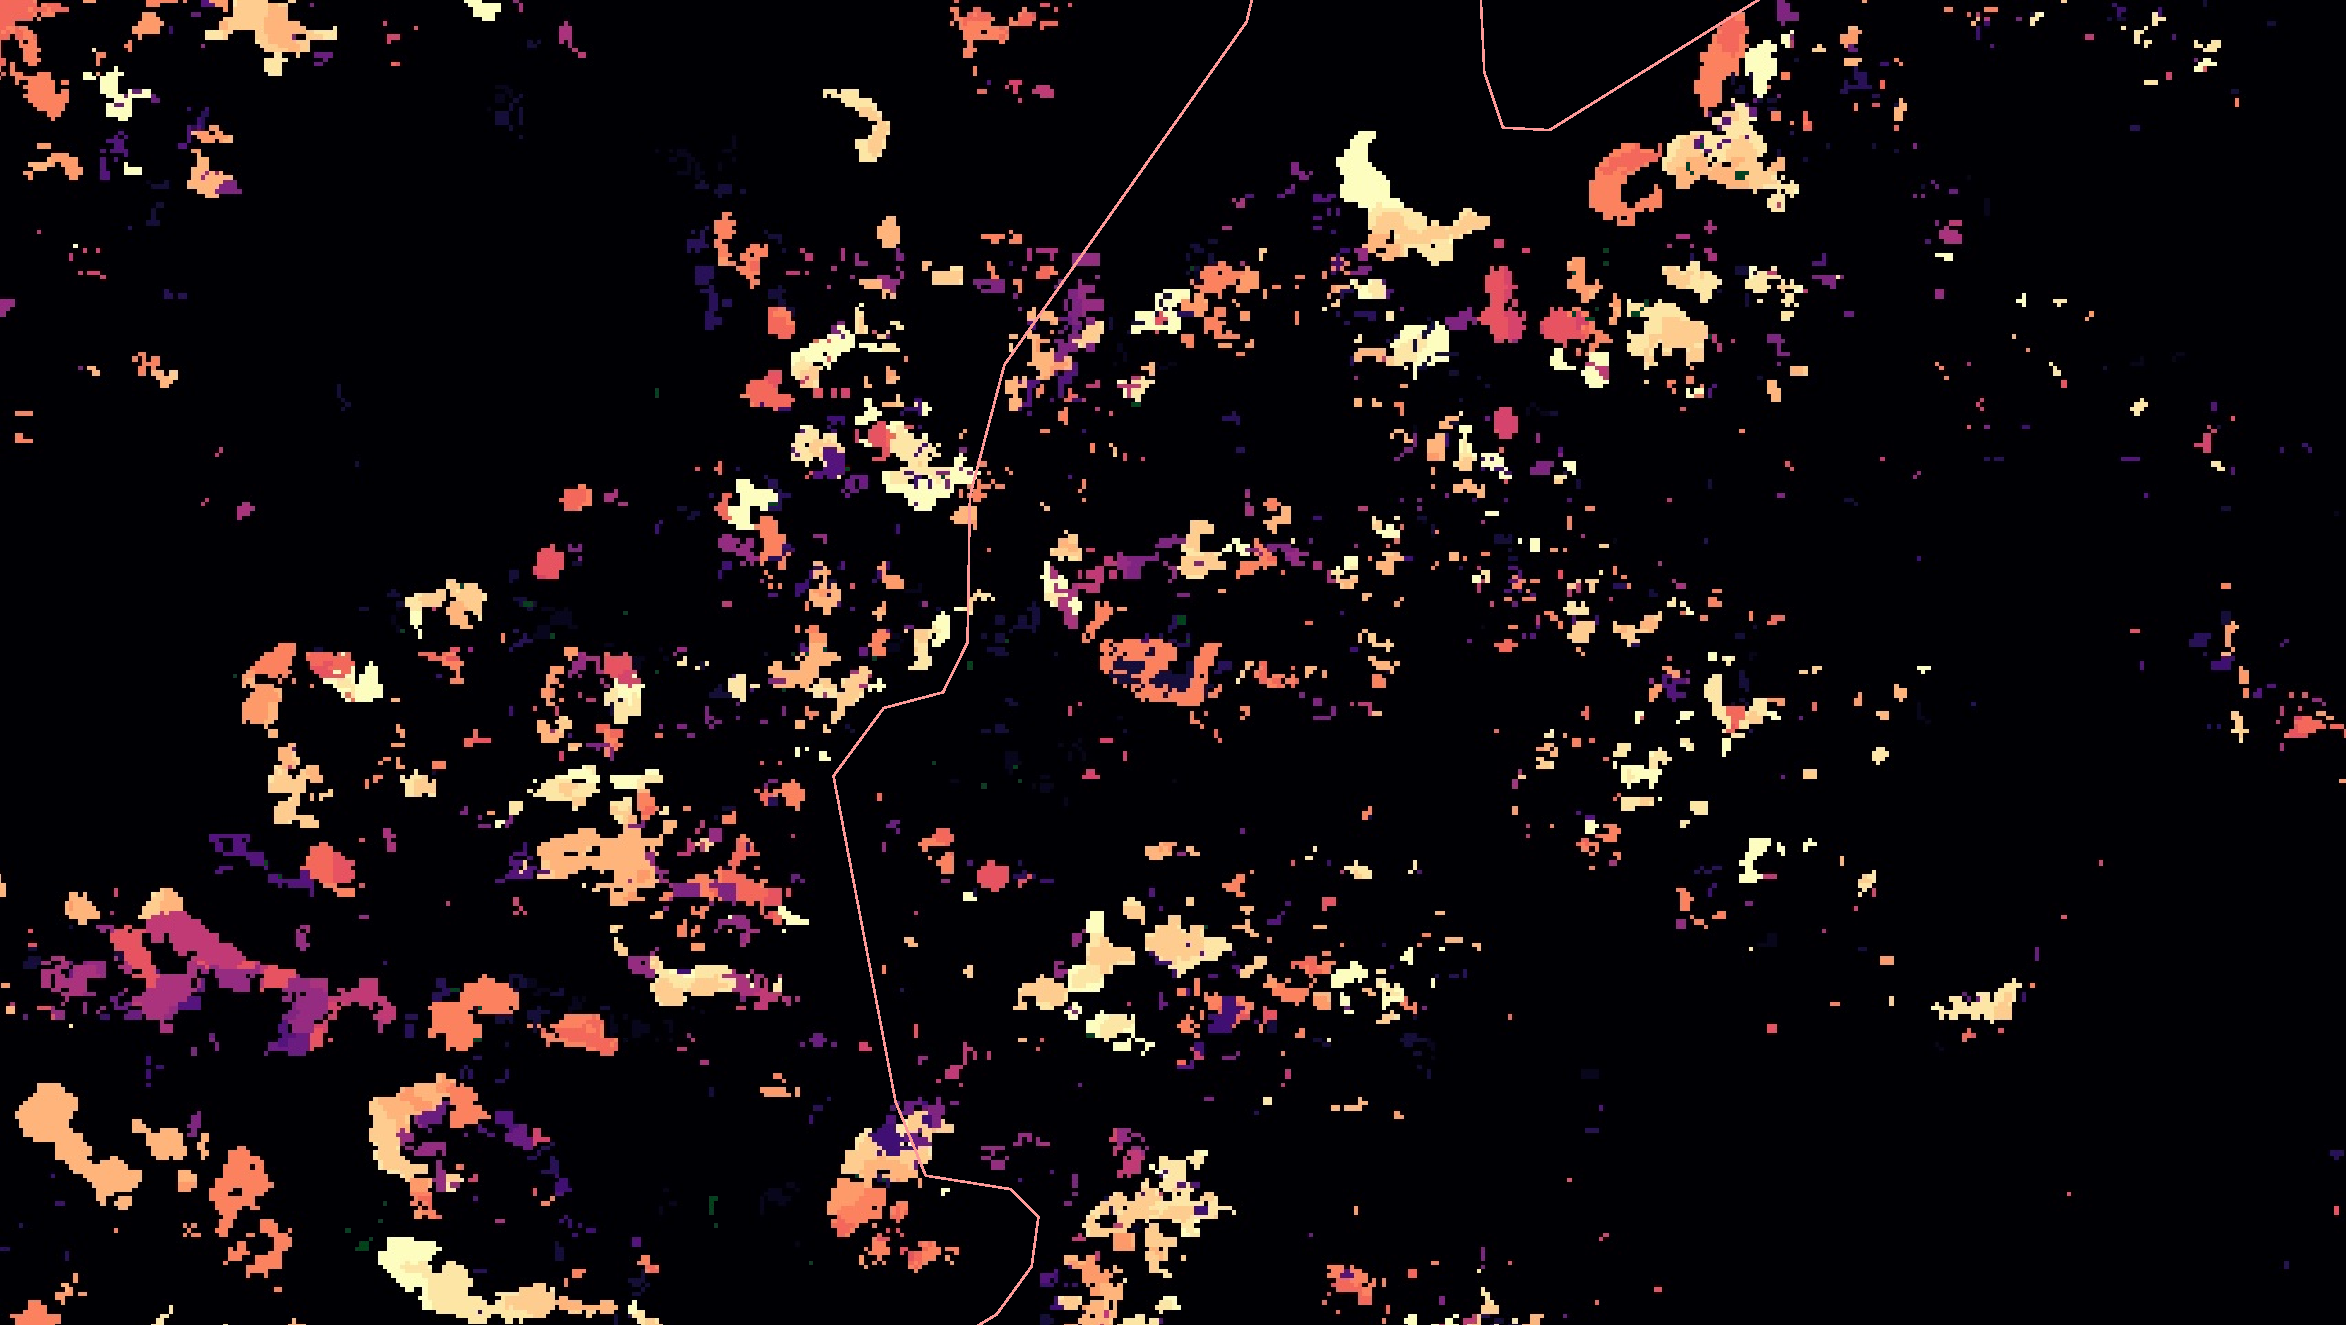
\includegraphics[width=6 in,angle=0]{Figs/loss_v_gain.pdf}}
\smallskip
\scriptsize
\emph{Notes}: 
%   \floatfoot{Notes: Forest loss (shaded red-to-yellow to indicate whether the cell was deforested in the past or recently) and gain (green) over the
%   entire sample period (2001-2017) in southern Jharkhand, India.
%   Forest loss is far more common than forest gain (which are a vanishingly small share; the only cells with forest gain are in dark green in the bottom left of the above figure) in the regions under
%   consideration, although India reportedly experienced net forest-gain
%   in the decades preceding the analysis \parencite{Foster2003-uz}.}
\end{minipage}
\end{center}
\end{figure}

% subsection deforestation_data (end)


\subsection{Administrative and Political Data} % (fold)
\label{sub:administrative_and_political_data}

%\footnote{Note that the deforestation raster is categorical: it reports an integer between 1 and 17 to correspond with the year in which a given cell was deforested. Therefore, the zonal statistic computation simply involves counting the number of cells in each village polygon that correspond with each year (for example, 3 in 2001, 5 in 2002, and so on), and merging it to the village data before reshaping to construct a panel.}
We use the \textcite{infomap2001indiamap} geocoded village-level Indian census to get boundaries of roughly 286,000 villages across the nine states where we conduct our analysis. For each village, we the aggregate the pixel-level deforestation data described above to the village level. To do this, we first compute zonal statistics for each village, which entails merging the pixel level raster dataset with the village polygons and counting the number of cells corresponding with each deforestation year in each village.  We then convert the number of deforested cells per year into hectares--a commonly used unit when discussing medium-scale areas--by multiplying the number of deforested cells in each year by $0.09$, since a hectare is $10,000 m^2$ and the area of a LANDSAT cell is $30\times30=900 m^2$. This gives us the dependent variable in terms of deforested area for each year.

% In sum, these data help us create a village level panel where we are able to measure the rate of deforestation for each village in India at the yearly level between 2000 and 2017. 

\subsection{Measuring Scheduled Areas} 

The construction of our treatment variable relies on manual coding of whether a village belongs to Scheduled Areas or not. To do this, we use information on the Government of India's Ministry of Tribal Affairs website. Each state releases official documents that list specific village names as Scheduled, or in cases where all villages within a block or district are Scheduled, the names of those blocks and districts are released.

While two states list village names (Andhra Pradesh and Rajasthan), the remaining states list block and district names. To remain consistent in our coding strategy across states, and to avoid human error that is more likely, we elected to code an entire block as Scheduled if \emph{any} village was designated as Scheduled within the block. Empirically, this approach is conservative because, while it accurately codes Scheduled Areas when all villages in a district and block are inside the treatment area, it codes some untreated villages within a block as treated -- that is, the resulting bias will be in the direction of zero. This coding is illustrated spatially in Figure \ref{fig:schmap} and a validation exercise that compares this coding with government issued maps is presented in \textcite{gulzar2019}.
%\begin{landscape}

% \todo[inline]{@apoorva please remove the header from the right panel. Can you also label the 0 and 1 and `Not Scheduled' and `Scheduled Areas' respectively? also, please confirm the caption below}



\begin{figure}[htbp!]
\begin{center}
\begin{minipage}{1 \linewidth}
\caption{\textbf{Forest cover in 2001 (left) and Scheduled Areas (right) in India}\label{fig:schmap}}	
\centerline{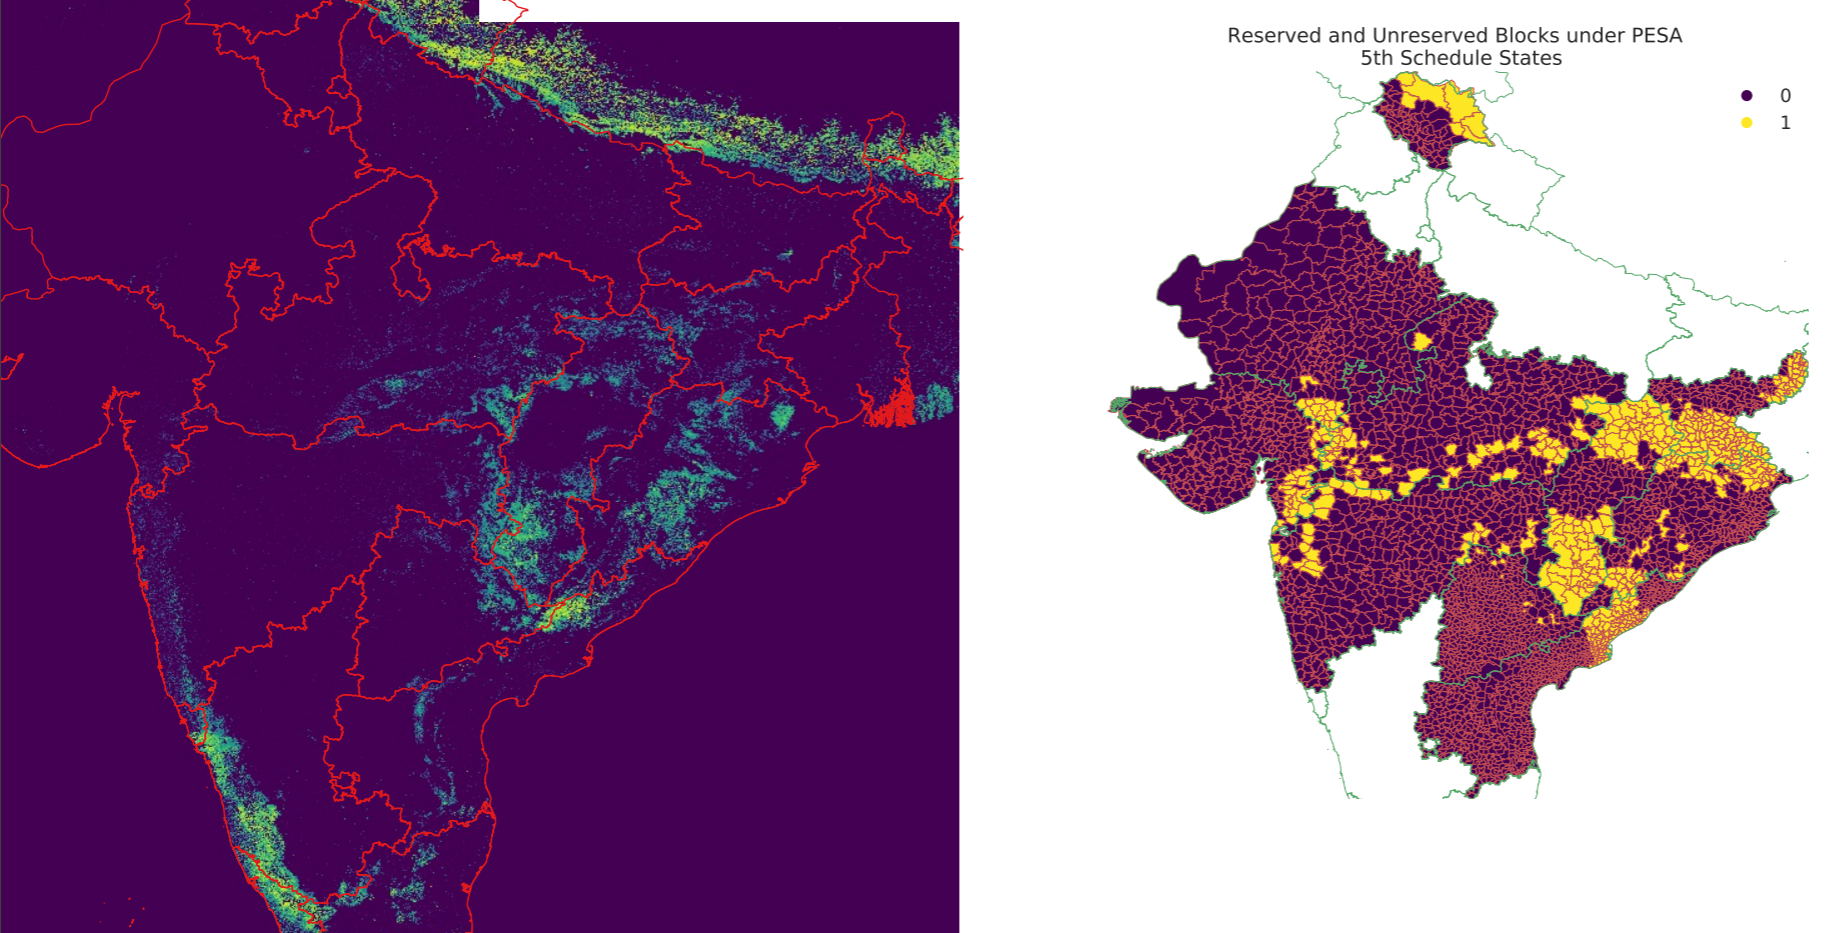
\includegraphics[width=6 in,angle=0]{Output/side_by_side.png}}
\smallskip
\scriptsize
\emph{Notes}: Left panel mosaiced from \textcite{Hansen2013-vk} where brighter shades correspond with more recent deforestation; Right panel reflects Scheduled Areas under the 5th Schedule of the Indian Constitution and neighbouring regions.
\end{minipage}
\end{center}
\end{figure}

%\end{landscape}
Once each village is coded as Scheduled or not as per the above procedure, we construct a switching indicator for Scheduled Areas in each state based on archival research of the first \emph{gram-panchayat} election in Scheduled Areas in accordance with PESA, where quotas were instituted for Scheduled Areas. We illustrate this timing in Figure \ref{fig:timing}. This restricts us to estimating treatment effects for 6 of the 9 treatment states because the remaining three implemented PESA before the first year in which forest data are available. 

We then merge these village level treatment timing data with the deforestation panel to finally arrive at our analysis sample, which is a balanced panel of roughly 300,000 villages over 17 years. Not all of these villages have any forest cover to begin with. We subset our main analysis to villages with above-median levels of forest cover in 2000 in our preferred specification Median forest cover for a village is our sample is 0.59 hectares and we analyse the sensitivity of our estimates to this cutoff.


\begin{figure}[htbp!]
\begin{center}
\begin{minipage}{1 \linewidth}
\caption{\textbf{PESA implementation timing for 9 states (plus neighbouring states close to border)} \label{fig:timing}}	
\centerline{\figinc{Output/PESA_adopt2.pdf}}
\smallskip
\scriptsize
\emph{Notes}: 
\end{minipage}
\end{center}
\end{figure}





\section{Empirical Strategy} % (fold)
\label{sec:empirical_strategy}

Since we have a panel dataset of each village with time-varying entry into the treatment, we begin the analysis with a standard generalised difference-in-differences design of the form:
\begin{equation}\label{base}
Y_{ist} = \tau \text{Scheduled Area}_{is} \times
\text{PESA Election Year}_{ist} +  \delta_i + \gamma_t +  \epsilon_{ist}
\end{equation}

where $i$ indexes villages, $s$ indexes state, and $t$ indexes years.
$Y_{ist}$ is the total area (in Hectares) deforested in village $i$ in
year $t$ , Scheduled Area $\times$ PESA Election Year$_{it}$ is a dummy
that for villages in scheduled areas in the year the first election
where PESA was implemented, $\delta_i$ is a village fixed effect, and $\gamma_t$ is a year fixed-effect.\footnote{Note that including village fixed effects means that other time invariant variables like the base term for Scheduled Areas cannot be included in the regression because of perfect collinearity.} $\tau$ corresponds with the causal effect of the introduction of PESA elections in Scheduled Areas.
The key value of the difference-in-differences design is that it includes village and year fixed effects which account for village-level unobserved characteristics that can directly affect deforestation rates, as well as common shocks (such as a national decline in economic activity) that might affect deforestation rates.  
We cluster standard errors by village in the main tables and examine robustness to more aggregated clustering, with the latter intended to account for potential spatial spillovers.  

% \todo[inline]{SG: put in citations for why we're following standard practice} 

The difference-in-differences design relies on the assumption of parallel trends, which in this context means that villages that fall in Scheduled Areas were on the same deforestation trajectories from those that were not in Scheduled Areas before the introduction of local elections under PESA. One might reasonably worry that this assumption might not be correct, and that simple village fixed effect, tantamount to having a single village-level intercept, may not capture potential differential trends. To account for this, we also introduce village level linear and quadratic time trends. These trends remove variation from the outcome by village that may potentially misattribute treatment effects to the policy if take-up was indeed non-random and related to the underlying village time trend of deforestation. Specifically, we estimate more flexible specifications of the following form:

\begin{equation}\label{ttrend}
Y_{ist} = \tau \text{Scheduled Area} \times \text{PESA Election Year}_{ist} +
\delta_i + \gamma_t + \delta_it + \delta_it^2 + \epsilon_{ist}
\end{equation}

where we have added additional terms $\delta_i t$ and $\delta_i t^2$ that are village-specific linear and quadratic time trends. In this specification, $\tau$ is identified off within-village variation, conditional on common year level unobservables \emph{and} village-level time trends for the entire sample. These village-specific time trends address confounding that might arise from secular changes in deforestation rates \emph{within any given village}; say, if a village has been steadily deforesting over time. 


Finally, one might reasonably worry that different state-level policies adopted at particular times may affect the outcome directly, which renders the estimate from common the year-fixed-effects specification biased. For example, a (hypothetical, unobserved) state-level policy implemented in Odisha in 2006 may have affected villages in Odisha alone; but having only year-fixed effects will not account for such unobservabed shocks. To address this, we run the following regression:
\begin{equation}\label{styfe}
Y_{ist} = \tau \text{Scheduled Area} \times \text{PESA Election Year}_{ist} +
\delta_i + \gamma_t + \xi_{st} + \epsilon_{ist}
\end{equation}

where $\xi_{st}$ is a vector of state-year fixed effects. These fixed effects control for unobservables that vary by state for each year and isolate the effect of PESA by comparing scheduled areas and non-scheduled areas within each state. In other words, this analysis pools across differences-in-differences estimates (wherein the treatment and control units are \emph{within} each state), and does not rely on the staggered adoption of the policy for causal identification. This is, to our mind, the most credible comparison wherein parallel trends are likely to hold.

% section empirical_strategy (end)

% ########  ########  ######  ##     ## ##       ########  ######
% ##     ## ##       ##    ## ##     ## ##          ##    ##    ##
% ##     ## ##       ##       ##     ## ##          ##    ##
% ########  ######    ######  ##     ## ##          ##     ######
% ##   ##   ##             ## ##     ## ##          ##          ##
% ##    ##  ##       ##    ## ##     ## ##          ##    ##    ##
% ##     ## ########  ######   #######  ########    ##     ######

\section{Results}\label{sec:Results} % (fold)

\subsection{Visualizing data}
As a first cut of our empirical approach, we visualize average (residualized) deforestation rates in Scheduled and non-Scheduled Areas for each year before and after PESA implementation (constructed relative to the year of implementation in each state) in Figure \ref{fig:schtrends}. We see that the rate of deforestation flattens substantially in scheduled areas following the implementation of the act.

% \todo[inline]{@apoorva, 1. can you remove the header from the figure below; 2. Make sure that the red and blue are printer friendly, or perhaps change the shape of the dots and lines to distinguish them,3. Add info on what the outcome has been residulized with respect to 4. maybe update the y axis to `Annual Deforestation in Hectares (residualized)' 5. Change y axis label to `Years since PESA Election'.}


\begin{figure}[htbp!]
\begin{center}
\begin{minipage}{1 \linewidth}
 \caption{\textbf{Average deforestation rate in Scheduled and Control Areas before and after the Implementation of the Panchayat Extension to Scheduled Areas Act}}	
\centerline{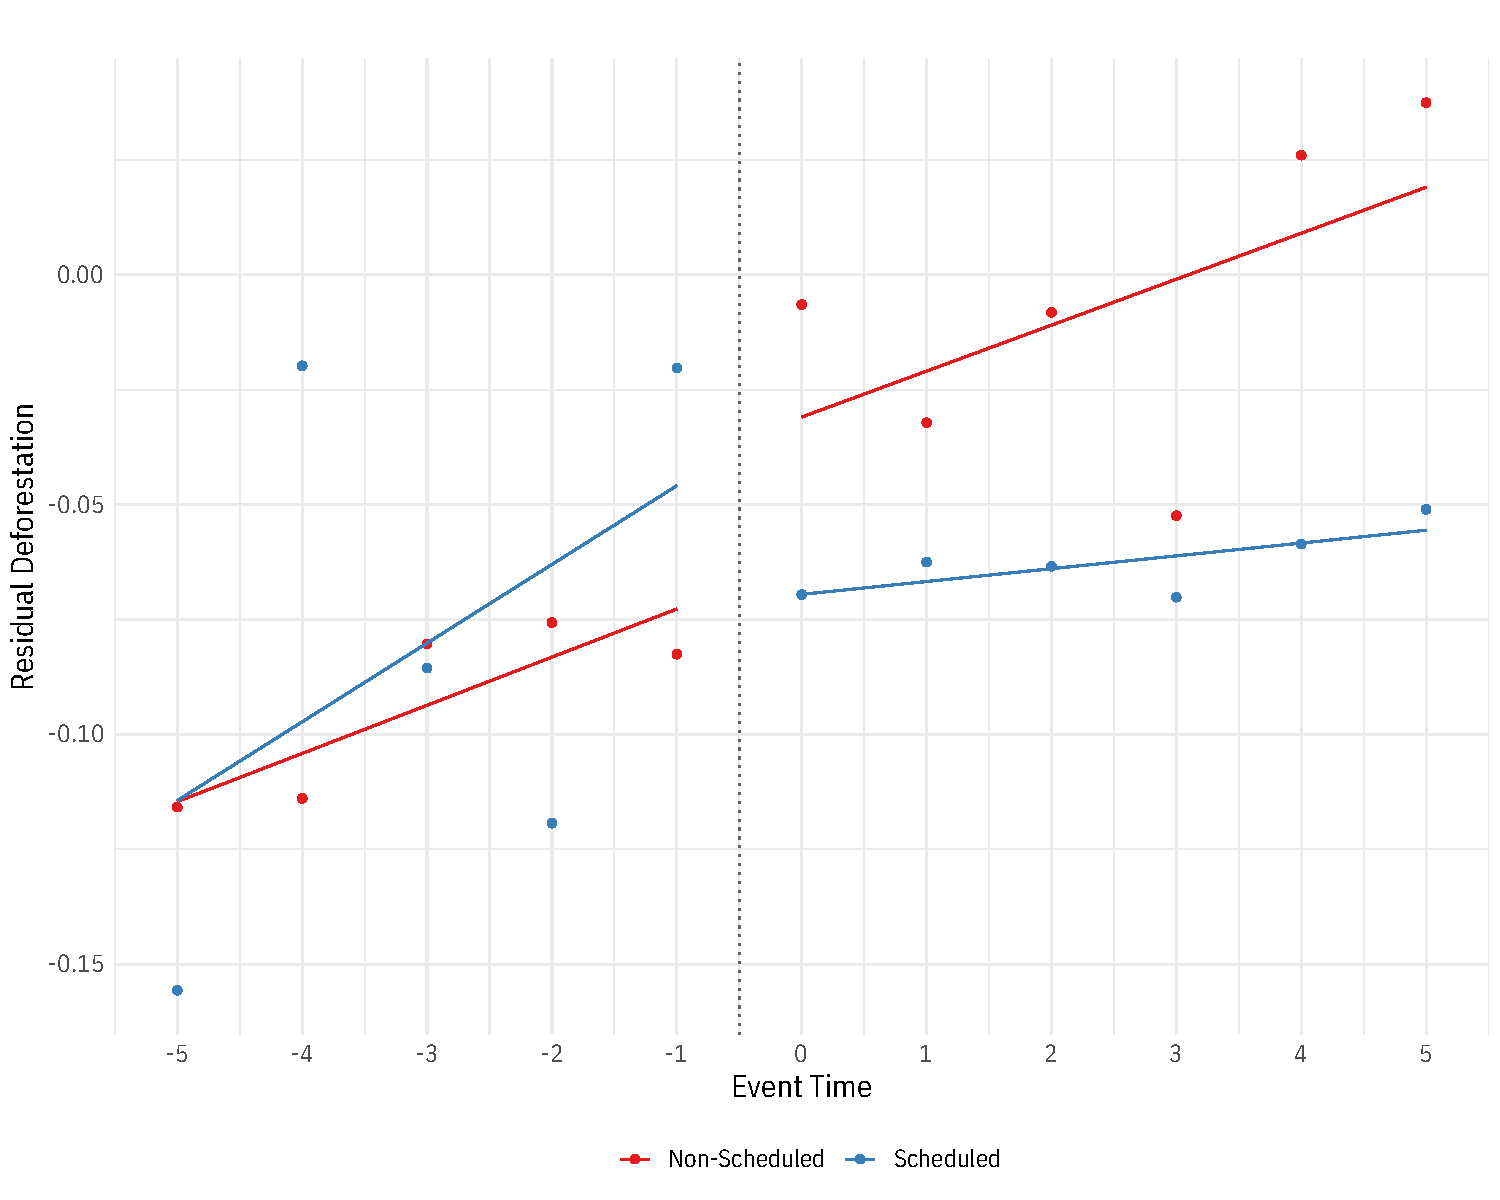
\includegraphics[width=5 in,angle=0]{Output/levels_time_trends.pdf}}
\smallskip
\scriptsize
\emph{Notes}: The outcome has been residualized for group means.
\end{minipage}
\end{center}
\end{figure}



\subsection{Main Effects}
Our main regression findings are reported in Table \ref{table:regres} below. Column 1 reports estimates of $\tau$ from \ref{base}, column 2 reports the estimates from \ref{ttrend}, and column 3 reports estimates from \ref{styfe}. As discussed above, for our primary analysis, we subset to villages with above median-levels of ex-ante forest cover, since including villages with effectively no forest cover mechanically biases estimates towards zero (since villages with no forest cover cannot have decreases in the rate of forestation), particularly because these are typically densely populated villages in `control' (non-scheduled) areas.


\begin{centering}
\begin{table}[!htbp] \centering
  \caption{Village Level Regressions}
  \label{table:regres}
  \input{Output/fe_estimates_ha_code_2011.tex}
\end{table}
\end{centering}

% \todo[inline]{Move the first three columns of Table 1 to the appendix, add a new column with the matched sample average effect which we can refer to when we discuss that later in the text}
% \eland

The estimated treatment effects are consistently large and negative.
In our preferred specification with state-year fixed effects (column 3) the implied reduction in the rate of deforestation is approximately $0.018$ hectares per village per year, $7\%$ on the overall mean of $0.22$. 
The difference in the
estimated treatment effect between the two-way fixed-effect estimate
(column 1), the specification that includes additional time-trends
(column 2), and state-year fixed effects (column 3) suggests that
there was plausibly positive selection into treatment. The
coefficients from the two specifications are in the same order of
magnitude and consistently have the same sign, which gives us
confidence that the time trends are absorbing confounding in terms of selection
into treatment.



% ########   #######  ########  ##     ##  ######  ########
% ##     ## ##     ## ##     ## ##     ## ##    ##    ##
% ##     ## ##     ## ##     ## ##     ## ##          ##
% ########  ##     ## ########  ##     ##  ######     ##
% ##   ##   ##     ## ##     ## ##     ##       ##    ##
% ##    ##  ##     ## ##     ## ##     ## ##    ##    ##
% ##     ##  #######  ########   #######   ######     ##

\paragraph*{Results are stronger when ex-ante forest cover is higher.} As a first robustness check of our main results, we vary the ex-ante forest cover cutoff for entry into our estimation sample and estimate \ref{styfe}
on the subset sample to test for whether the coefficient is sensitive to the choice of ex-ante forest cutoff. The results are presented in Figure
\ref{fig:cutoff_plot}. The estimate for the 5$^{th}$ decile and up corresponds with our primary specification in table \ref{table:regres}.


\begin{figure}[htbp!]
\begin{center}
\begin{minipage}{1 \linewidth}
\caption{\textbf{Treatment Effects as a Function of Ex-Ante Forest Cover Cutoffs}\label{fig:cutoff_plot}} 	
\centerline{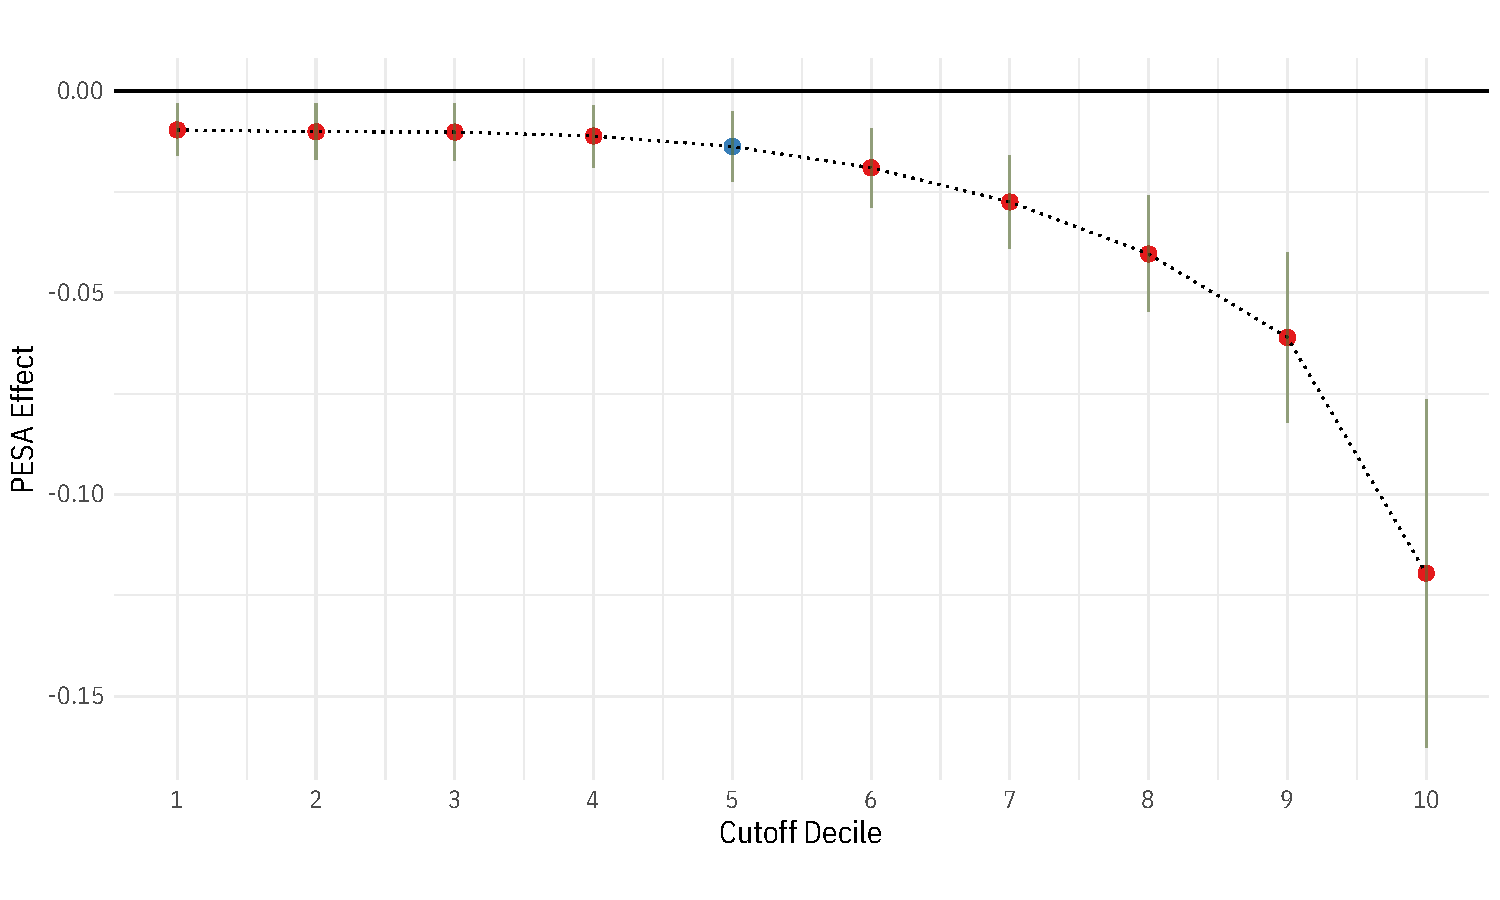
\includegraphics[width=5 in,angle=0]{Output/varying_cutoff2.pdf}}
\smallskip
\scriptsize
\emph{Notes}: The figure reports treatment effect estimates with specification \ref{styfe}., with SE estimates clustered by village. The point in blue corresponds with the estimate in column (3) in ~\ref{table:regres}. 
\end{minipage}
\end{center}
\end{figure}


\paragraph*{Results are consistent with an alternative source of forest data.} We estimate the same specifications as in section ~\ref{sec:empirical_strategy} using outcome data derived from an alternate source of forest cover data: the Vegetation Continuous Fields data aggregated by \textcite{almn2019}. This data provides annual tree cover from 2000-2014 in the form of the percentage of each pixel under forest cover \parencite{Sexton2013-xx}. Since the outcome in these regressions is the vegetation index, a positive coefficient indicates a net positive effect on forest levels. A major drawback of these data, however, is that they are derived from a different satellite with a coarser resolution than our primary data ($250\times250m$ cells) and therefore some villages' indices are derived from a small handful of measurements. Nevertheless, the results serve as a useful robustness check and validate our main findings. The results are reported in section \ref{sub:vcf_est}


\paragraph*{Results are consistent with more aggregated clustering.}
Finally, in table \ref{table:regres2}, we report results from the main specifications clustered at the sub-district to account for both spatially correlated errors within Subdistricts (also known as Tehsils, administrative units comprised of multiple blocks, which in turn are comprised of multiple villages), and serial autocorrelation in errors. Clustering at a large administrative unit is somewhat comparable to (and more conservative) than estimating Conley standard errors with a large bandwidth. This massively increases the standard errors in specifications with many additional parameters (such as village time trends and state-year FEs), but the two-way-FE specification remains significant at the 1\% level.

% section robustness_checks (end)



\subsection{Event study design} % (fold)
\label{sub:dynamic_treatment_effects}

Next, we report yearly treatment effects which present an intuitive method of performing a Granger Causality test, wherein the leads should be relatively insignificant and moderate in size, while the contemporaneous and lagged effects ought to be large if the PESA policy is indeed the cause of the changes in deforestation outcomes. To do this, we estimate the following model:

\begin{equation}\label{granger}
 Y_{ist} = \delta_i + \gamma_t + \delta_it + \delta_it^2  +
\sum_{\phi=-1}^m \tau_{-\phi}
D_{i, t - \phi} + \sum_{\phi=0}^q \tau_{+\phi} D_{i,t+\phi}
+ \epsilon_{ist}   
\end{equation}

 which includes leads and lags of the treatment dummy to decompose the treatment effect by each year preceding and following the switch from pre- to post-PESA. We take the year immediately preceding the treatment as the omitted baseline year of comparison to avoid saturating the model.
 %\parencite[Appendix G]{cengiz2019effect}. 
 
 The results are reported graphically in Figure \ref{fig:autor_plot} for different sub-samples of the data, in increasing order of ex-ante forest levels, with the bottom left (6th Decline and up) panel corresponding with the main analysis sample in the previous section.  We observe some anticipation effects (based on the significant negative coefficient for $-2$), as can be expected from a publicly announced policy, but the bulk of effects are large and persistent following the treatment year. Finally, consistent with Figure \ref{fig:cutoff_plot}, the treatment effects are larger when we restrict the sample to higher ex-ante forest cover.

\begin{figure}[htbp!]
\begin{center}
\begin{minipage}{1 \linewidth}
\caption{\textbf{Dynamic Treatment Effects of PESA Adoption} \label{fig:autor_plot}} 	
\centerline{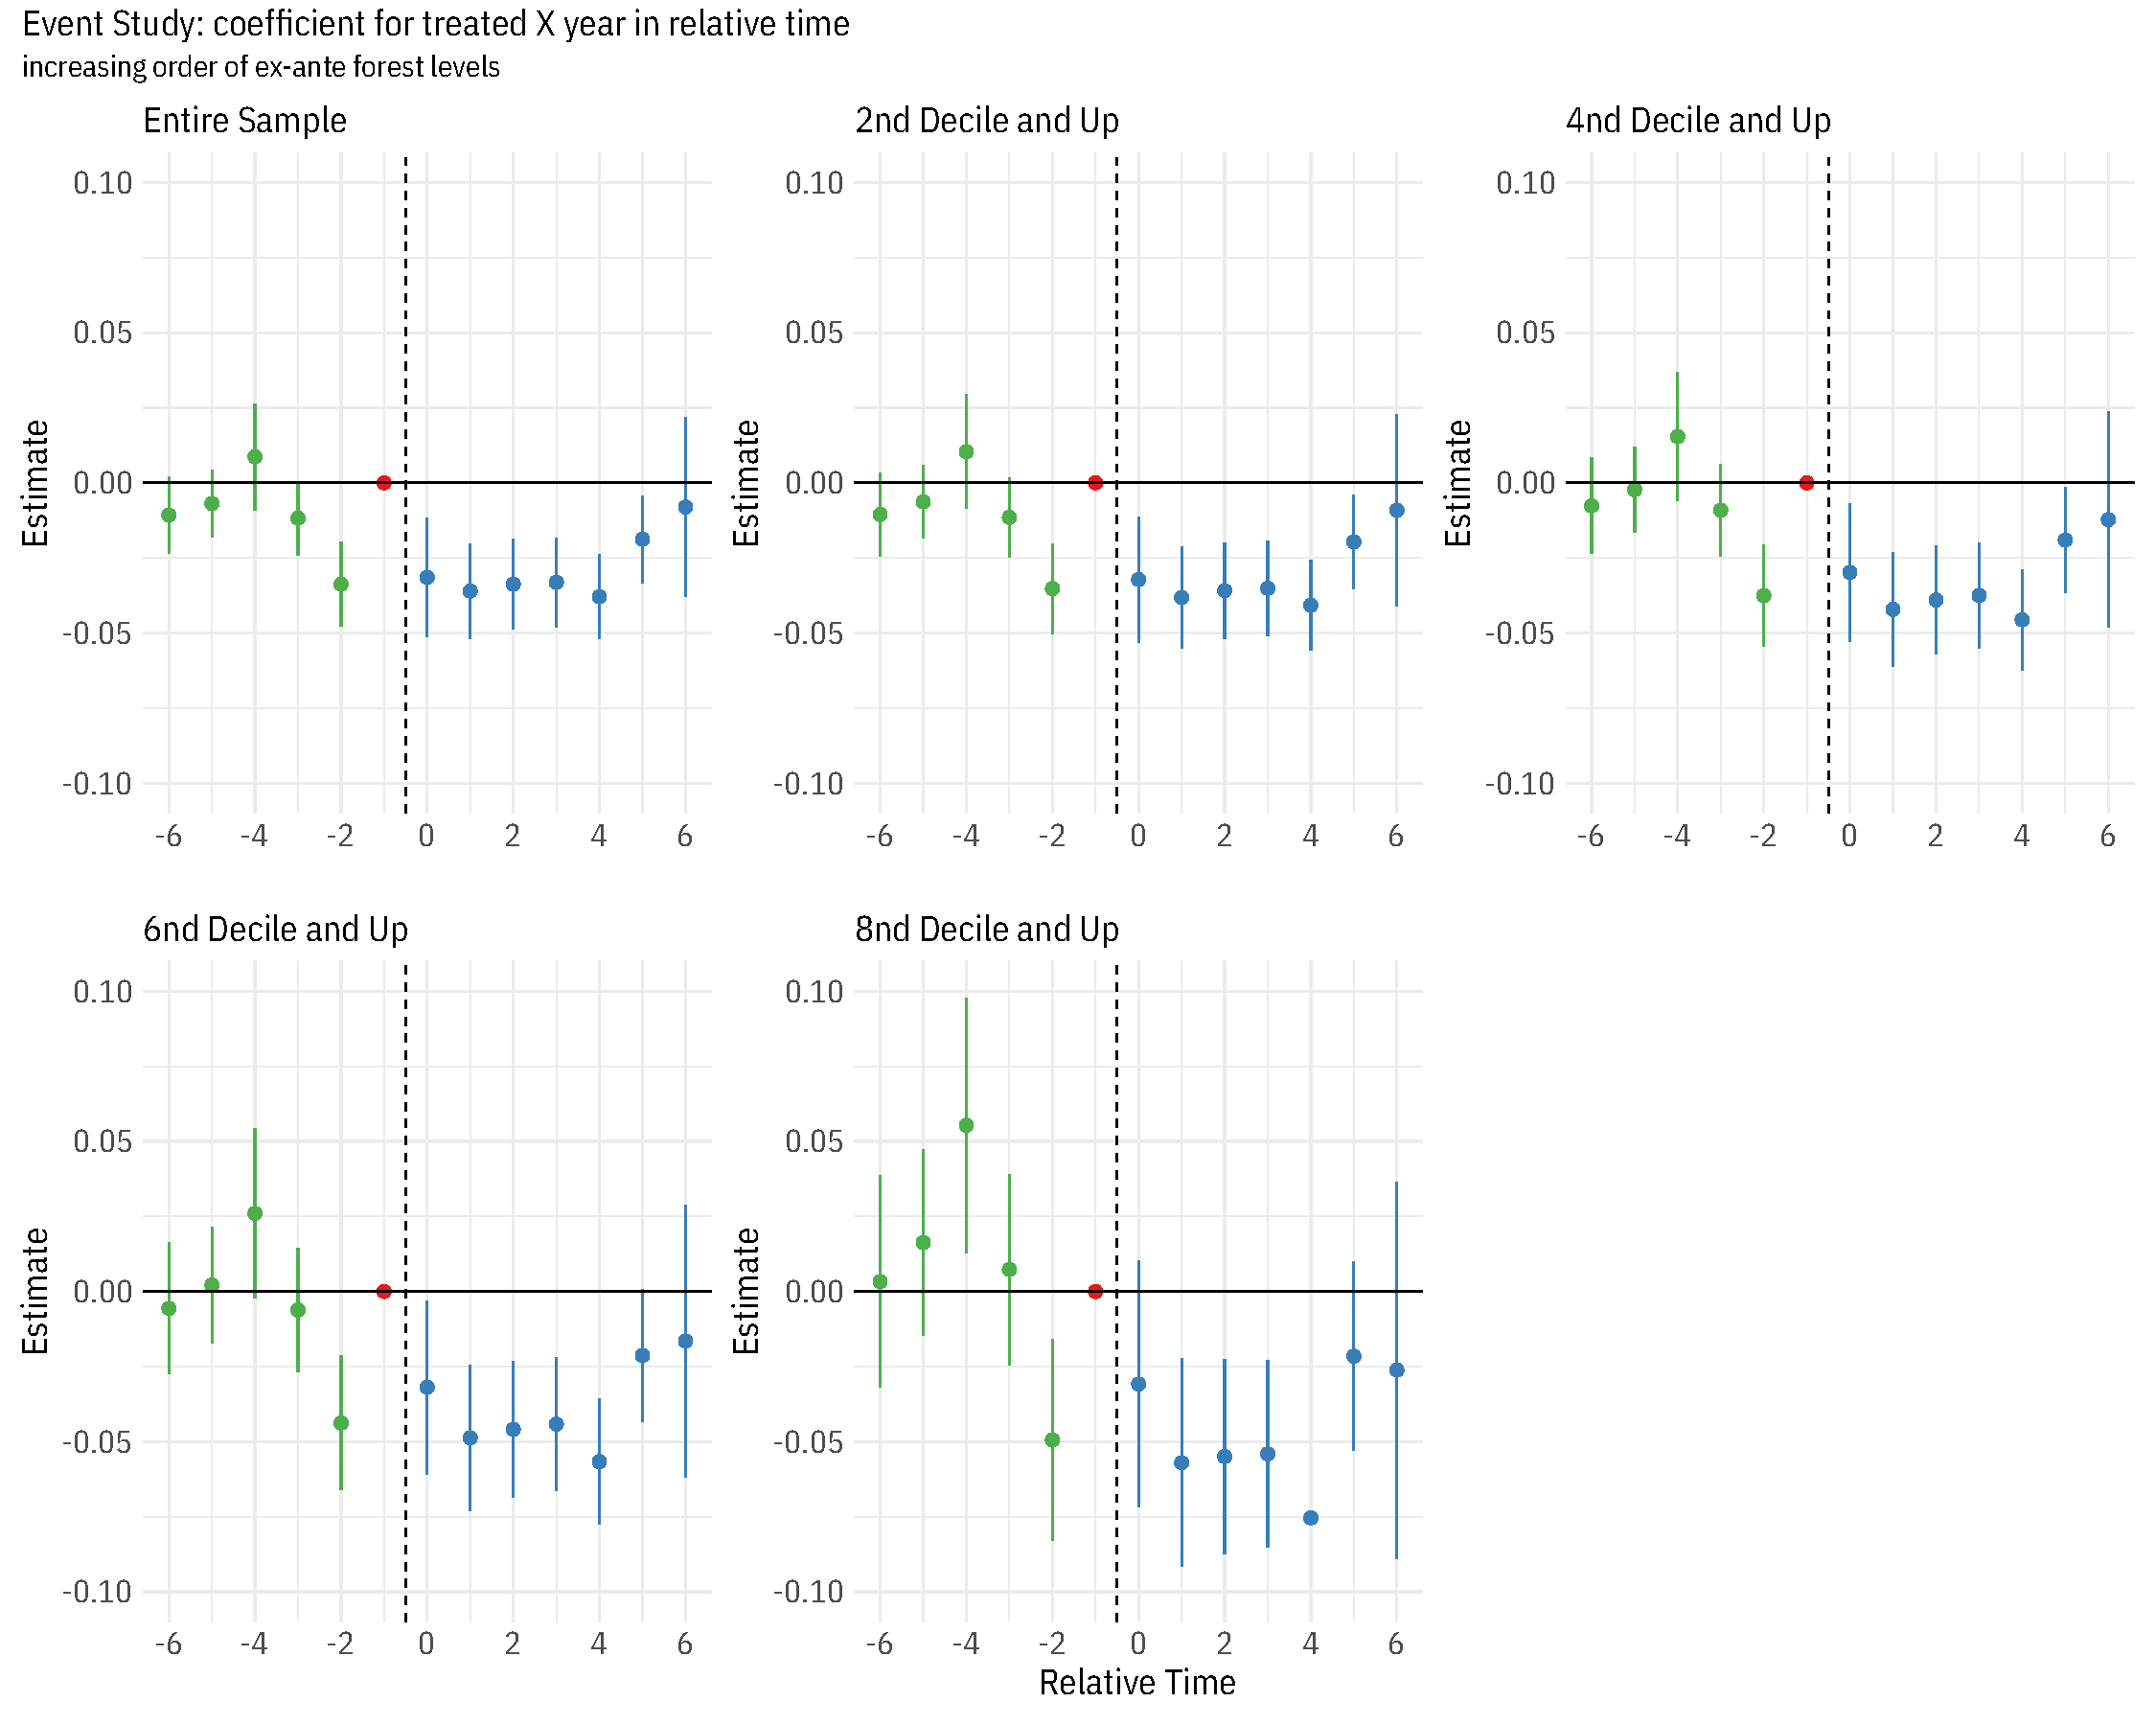
\includegraphics[width=7.5 in,angle=0]{Output/Dyn_treat_eff_big.pdf}}
\smallskip
\scriptsize
\emph{Notes}: This figure presents result from the event study regression.
\end{minipage}
\end{center}
\end{figure}


To further account for potential differences in pre-trends across the two groups, we perform a matched difference-in-differences analysis wherein we exact-match on State and ex-ante forest cover decile and coarse match on the outcome variable (deforestation area) for the villages in our sample, as suggested by \textcite[]{Imai2019-kp}. This allows us to estimate treatment effects on the matched sample which we report in Figure \ref{fig:panelmatch}. This analysis restricts the sample to treatment and control villages that are in the same state, have comparable amounts of ex-ante forest cover in 2000 (that is, they are in the same decile for ex-ante forest cover), and have a similar rate of deforestation for 4 years prior to PESA implementation (which mechanically rules out differential pre-trending by sub-setting to the best match to treatment villages). We report a balance-test for pre-treatment deforestation in Figure \ref{fig:panelmatchbal} and conclude that the matched samples are well-balanced (with the comparison in SD motivated by \textcite[]{imbens2015causal}, who argue that standardised balance tests are advisable over comparisons in raw measures).

In summary, we find that the treatment effect appears precisely in the election year and then stabilises to a lower rate in subsequent years (which is understandable given that our outcome is measured as a \emph{rate} and not a \emph{level} of deforestation). This provides stronger evidence to justify a causal interpretation of the observed decline in deforestation rate following the introduction of PESA. 


\begin{figure}[htbp!]
\begin{center}
\begin{minipage}{1 \linewidth}
  \caption{\textbf{Dynamic Treatment Effects of PESA Adoption using matched villages}}
  \label{fig:panelmatch}	
\centerline{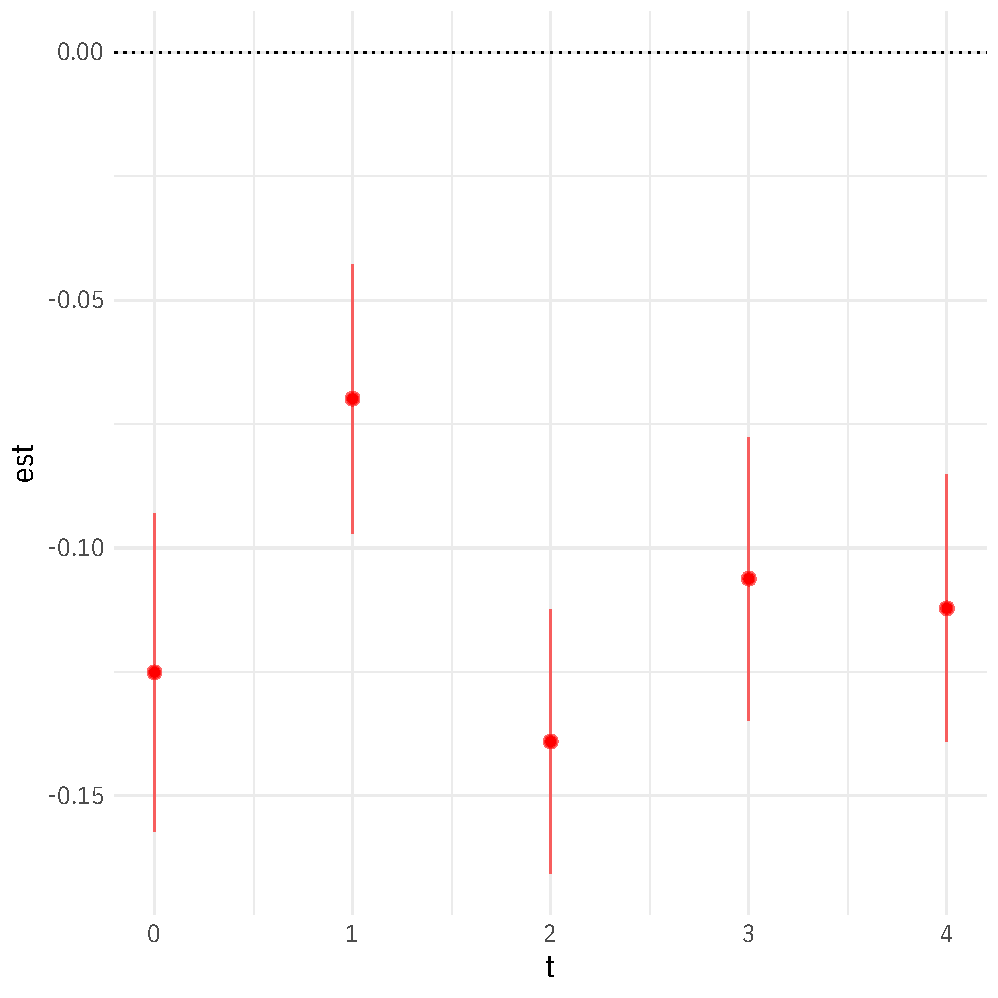
\includegraphics[width=3 in,angle=0]{Output/panelmatch_fig.pdf}}
\smallskip
\scriptsize
\emph{Notes}: This figure reports results from a matched sample. We used exact matching on state and ex-ante forest decile and coarse matched the sample on deforestation (outcome) on the 4 preceeding periods to PESA implementation. Matching is performed using PanelMatch.
\end{minipage}
\end{center}
\end{figure}




\subsection{Mechanisms} % (fold)
\label{ssub:possible_mechanisms}

One of the hypothesised mechanisms for the reduction in deforestation is that ST politicians are able to gain political power in gram panchayat elections and subsequently reduce deforestation. As such, it follows that we should see larger treatment effects in areas that have an ex-ante ST plurality because their preferences of renewable resources are most likely to get represented when elites are likely to be selected from their communities. To test this mechanism, we first define ST Majority as ST Population Share - Non-ST Population Share, which is distributed on $[-1, 1]$ (villages with no ST have -1 ST Majority, while villages that are exclusively ST have 1). We then interact the treatment indicator in \ref{styfe} with bins of the ST majority variable to flexibly capture the treatment effect as a function of ST majority. This allows the treatment effect to vary non-linearly by bin (as suggested by \parencite{hainmueller2019much}) as opposed to imposing a strong linear form using a linear interaction term. 

We fail to rule out the null of uniform treatment effects as a function of ST composition, as reflected in ~\ref{fig:intflex_stmaj}. Interpreting interior values is somewhat challenging given the distribution of ST majorities, which is highly bimodal: they are either a negligible share of the electorate or constitute a plurality, see \ref{fig:st_share_dist}), and as a result, coefficients for intermediate values are estimated imprecisely. Furthermore, since one of the key criteria for PESA designation was ST population share, treatment overlap is weak over the distribution of the ST majority share.


% \begin{centering}
% \begin{table}[!htbp] \centering
%   \caption{Regressions with ST Plurality Interaction}
%   \label{table:regres}
%   \input{Output/plurality_test_regs.tex}
% \end{table}
% \end{centering}


\begin{figure}[htbp!]
\begin{center}
\begin{minipage}{1 \linewidth}
  \caption{\textbf{Treatment effects by ST majority}\label{fig:intflex_stmaj}	}
  
\centerline{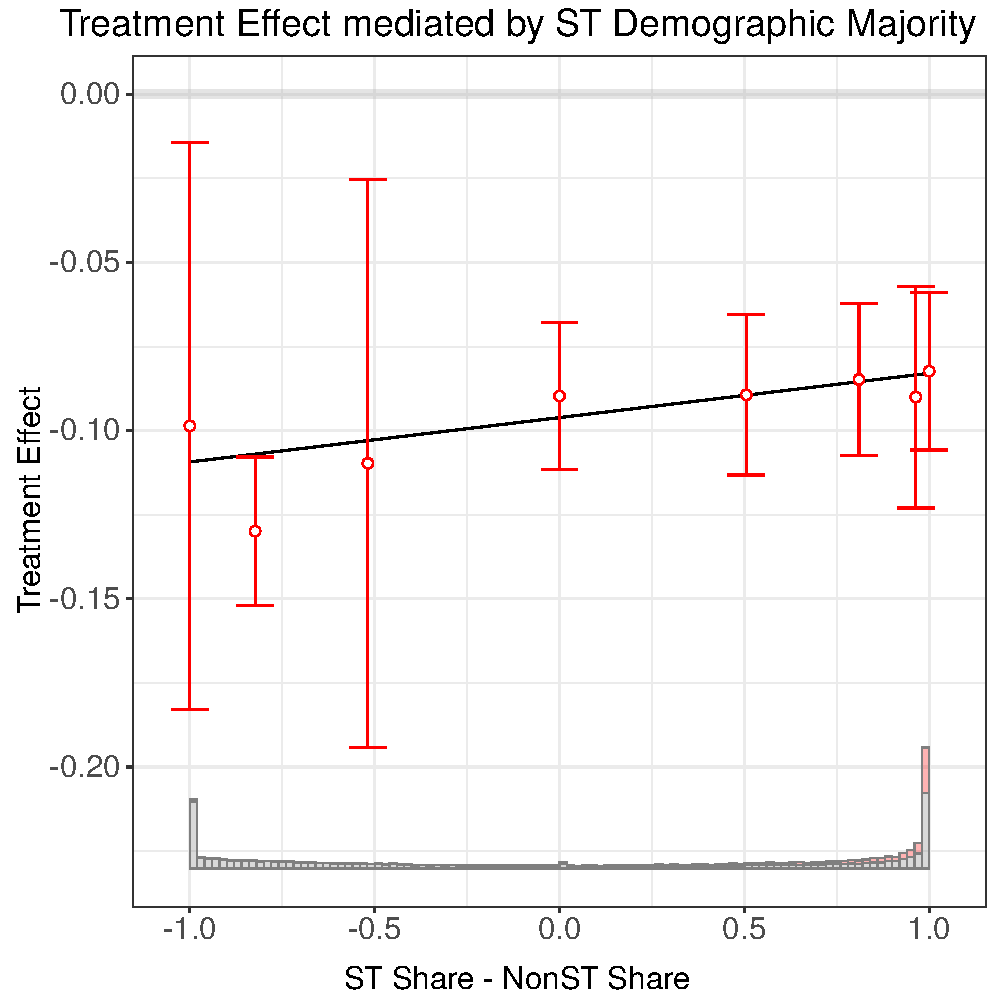
\includegraphics[width=3 in,angle=0]{Output/Interflex_stmaj.pdf}}
\smallskip
\scriptsize
\emph{Notes}: 
\end{minipage}
\end{center}
\end{figure}


Another hypothesised mechanism, closely related to the model proposed in \textcite{Burgess2012-hk}, is that villages rich in natural resources were previously unable to regulate resource extraction because of lack of political power for marginalized communities are now able to do so following the implementation of ST political quotas. To test this, we use data from the Indian Mining Census, compiled by \textcite{asher2019rent}. The mining census lists every known mine and its geolocation and type (see Figure \ref{fig:mine_map}), which allows us to compute the distance from every village to every mine. We then use the minimum of these distances as a mediator for the regression to examine if treatment effects are indeed stronger for villages that are located close to mining sites. We decompose the treatment effect by tercile of distance to the closest mine in the regression specification in Table \ref{table:regres} and by every 10 km bin in Figure \ref{fig:mining_plot}. For completeness, we also report the treatment effect decomposed by distance to every mine type with sufficient data in Appendix Figure \ref{fig:mine_het_te}.

\begin{centering}
\begin{table}[!htbp] \centering
  \caption{Sub-group Analysis by Distance to Mines}
  \label{table:regres}
  
\begin{table}[!htbp] \footnotesize \centering 
  \caption{Treatment Effects on Annual Deforestation by Distance to Nearest Mine. } 
  \label{table:regresmine} 
\begin{tabular}{@{\extracolsep{0pt}}lccccc} 
\\[-1.8ex]\hline \\[-1.8ex] 
\\[-1.8ex] & \multicolumn{5}{c}{Annual Deforestation in Hectares} \\ 
\\[-1.8ex] & (1) & (2) & (3) & (4) & (5)\\ 
\hline \\[-1.8ex] 
 Scheduled $\times$ PESA $\times$ 1st Tercile & $-$0.093$^{***}$ & $-$0.043$^{***}$ & $-$0.025$^{**}$ & $-$0.079$^{***}$ &  \\ 
  & (0.010) & (0.014) & (0.010) & (0.015) &  \\ 
  Scheduled $\times$ PESA $\times$ 2nd Tercile & $-$0.103$^{***}$ & $-$0.034$^{**}$ & $-$0.026$^{**}$ & $-$0.077$^{***}$ &  \\ 
  & (0.012) & (0.016) & (0.011) & (0.016) &  \\ 
  Scheduled $\times$ PESA $\times$ 3rd Tercile & $-$0.052$^{***}$ & $-$0.004 & 0.018 & $-$0.031 &  \\ 
  & (0.017) & (0.026) & (0.017) & (0.025) &  \\ 
  Scheduled $\times$ PESA &  &  &  &  & $-$0.061$^{***}$ \\ 
  &  &  &  &  & (0.012) \\ 
  Scheduled $\times$ PESA $\times$ Mine within 5 km &  &  &  &  & $-$0.052$^{**}$ \\ 
  &  &  &  &  & (0.020) \\ 
 Village FE & $\checkmark$ & $\checkmark$ & $\checkmark$ & $\checkmark$ & $\checkmark$ \\ 
Year FE & $\checkmark$ & $\checkmark$ &  &  &  \\ 
Village TT &  & $\checkmark$ &  & $\checkmark$ & $\checkmark$ \\ 
State $\times$ Year FE &  &  & $\checkmark$ & $\checkmark$ & $\checkmark$ \\ 
Dep. Var. Mean & 0.22 & 0.22 & 0.22 & 0.22 & 0.22 \\ 
N. Villages & 52776 & 52776 & 52776 & 52776 & 52776 \\ 
N & 897,192 & 897,192 & 897,192 & 897,192 & 897,192 \\ 
\hline \\[-1.8ex] 
\multicolumn{6}{l}{$^{*}$p $<$ .1; $^{**}$p $<$ .05; $^{***}$p $<$ .01} \\ 
\multicolumn{6}{l}{Cluster-Robust Standard Errors (by village)} \\ 
\multicolumn{6}{l}{Terciles are defined based on the distribution of village distances to mines,} \\
\multicolumn{6}{l}{ with the 1$^{st}$ being $1-33$ percentile, and so on.}
\end{tabular} 
\end{table} 

\end{table}
\end{centering}


% The Mining Census lists the total production
% and value of various minerals extracted in each district for every
% year since the 1981, and we use pre-treatment production for each
% district found in the mineral database for the 10 highest value
% minerals \footnote{These include gold, coal, bauxite, copper and so
% on. Subsetting by value omits some seemingly less relevant minerals,
% such as clay. Using the presence of any of the entire of the original
% extensive list of minerals labels well over 90\% villages as `mining
% potential', which leaves us with little variation to work with. The
% results are qualitatively similar when employing slightly more
% restrictive (presence of 5 most high value minerals) and inclusive
% definitions of mining potential} to classify districts as either high
% or low mining potential. We then estimate the three specifications above
% including an interaction with an indicator for mining potential in the district.

In both the tercile regressions as well as distance band regressions, the treatment effect is strongest in villages that are close to mines.  This suggests that reduced mining, potentially through village council oversight over mining in the forests, might be a possible mechanism for the observed decrease in deforestation, though our data do not allow for a direct test of this.

\begin{figure}[htbp!]
\begin{center}
\begin{minipage}{1 \linewidth}
  \caption{\textbf{Treatment effects by Distance to Mines}}
  \label{fig:mining_plot}	
\centerline{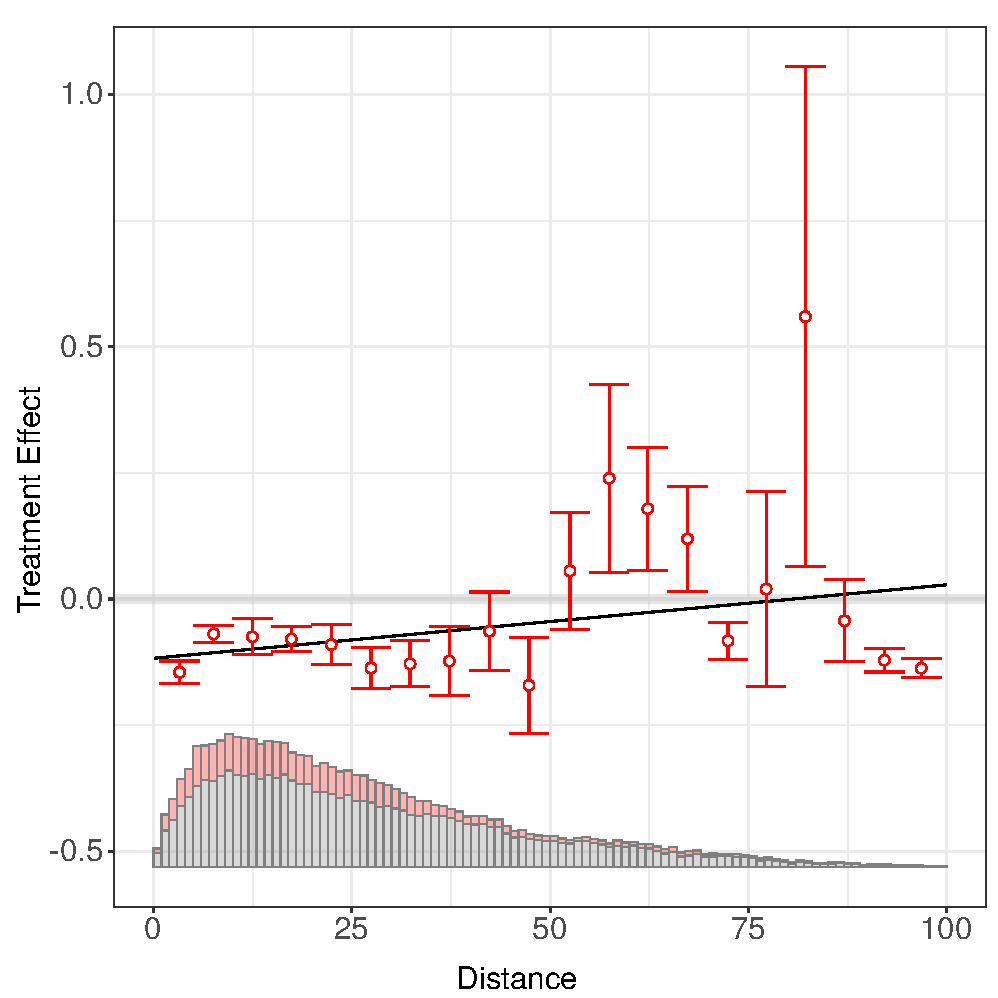
\includegraphics[width=4 in,angle=0]{Output/Interflex_main.pdf}}
\smallskip
\scriptsize
\emph{Notes}: 
\end{minipage}
\end{center}
\end{figure}





\pagebreak


% subsubsection possible_mechanisms (end)


%  ######   #######  ##    ##  ######
% ##    ## ##     ## ###   ## ##    ##
% ##       ##     ## ####  ## ##
% ##       ##     ## ## ## ## ##
% ##       ##     ## ##  #### ##
% ##    ## ##     ## ##   ### ##    ##
%  ######   #######  ##    ##  ######


\section{Conclusion} % (fold)
\label{sec:conclusion}

In summary, we find that a law introducing local government quotas for disadvantaged groups substantially reduced the rate of deforestation in Indian villages. We provide suggestive evidence in favour of an electoral control mechanism -- that PESA reservations resulted in ST politicians gaining greater electoral control and in turn reducing resource extraction. We hypothesise that the election of ST leaders to local councils improved enforcement, thereby reflecting the strong preservation norms among the scheduled tribes in village policy. Endowing political and bureaucratic power at administrative units congruent with networks at which informal norms of preservation exist may improve the effectiveness of environmental preservation -- by lowering enforcement costs -- and adding administrative frictions that render illegal overuse more costly.

We find evidence that local governments can be effective in promoting environmental protection, especially when key stakeholders, such as ST in India, are included pro-actively. This finding runs counter to the argument that administrative unit proliferation and decentralisation create incentives for over-extraction by exacerbating collective action problems. By contrast, we find suggestive evidence that collective action problems were overcome by informal institutions, within identity-based communities, that enforced norms of sustainable resource use.


% section conclusion (end)

\pagebreak

%%%%%%%%%%%%%%%%%%%%%%%%%%%%%%%%%%%%%%%%%%%%%%%%%%%%%%%%%%%%%

% \renewcommand{\mkbibnamefamily}[1]{\textsc{#1}}
\printbibliography

\newpage
\renewcommand{\thetable}{A\arabic{table}}
\renewcommand{\thefigure}{A\arabic{figure}}
\setcounter{table}{0}
\setcounter{figure}{0}

\appendix

The computation in this paper was performed in R, Python, and Stata using the following libraries:
\textcite{wickhamGgplot2ElegantGraphics2010}, 
\textcite{wickhamDplyrGrammarData2015}, 
\textcite{gaureLfeLinearGroup2013}, 
\textcite{mckinneyPandasFoundationalPython2011}, 
\textcite{jordahlGeoPandasPythonTools2014}, 
\textcite{waltNumPyArrayStructure2011},
\textcite{hunterMatplotlib2DGraphics2007},
\textcite{hainmueller2019much}, 
\textcite{correia2019reghdfe}


\section{Additional Tables}

\subsection{Summary Statistics} % (fold)
\label{ssub:summary_statistics}



\begin{tabular}{@{\extracolsep{5pt}}lccccccc} 
\\[-1.8ex]\hline 
\hline \\[-1.8ex] 
Statistic & \multicolumn{1}{c}{N} & \multicolumn{1}{c}{Mean} & \multicolumn{1}{c}{St. Dev.} & \multicolumn{1}{c}{Min} & \multicolumn{1}{c}{Pctl(25)} & \multicolumn{1}{c}{Pctl(75)} & \multicolumn{1}{c}{Max} \\ 
\hline \\[-1.8ex] 
\# households & 285,182 & 333.700 & 1,833.000 & 1 & 80 & 316 & 248,162 \\ 
Population & 285,182 & 1,561.000 & 8,455.000 & 10 & 374 & 1,501 & 977,771 \\ 
Scheduled & 285,182 & 0.187 & 0.390 & 0 & 0 & 0 & 1 \\ 
2000 Forest Index (Max) & 285,182 & 28.300 & 27.570 & 0 & 6 & 45 & 100 \\ 
200 Forest Index (Mean) & 285,182 & 3.167 & 9.197 & 0.000 & 0.007 & 0.684 & 89.100 \\ 
Number of Cells & 285,182 & 7,728.000 & 12,621.000 & 5 & 2,271 & 9,156.0 & 1,236,411 \\ 
ST Share & 285,182 & 0.282 & 0.364 & 0.000 & 0.000 & 0.549 & 1.000 \\ 
SC Share & 285,182 & 0.143 & 0.178 & 0 & 0.002 & 0.2 & 1 \\ 
\hline \\[-1.8ex] 
\end{tabular} 

% subsubsection summary_statistics (end)

\subsection{Auxiliary Regression Estimates}

\clearpage

\begin{centering}
\begin{table}[!htbp] \centering
  \caption{Village Level Regressions clustered at sub-district level}
  \label{table:regres2}
  \input{Output/fe_estimates_ha_sub_dist.tex}
    % \include{Output/fe_estimates_stata}
\end{table}
\end{centering}

\begin{centering}
\begin{table}[!htbp] \centering
  \label{table:fullsamp}
  \caption{Full sample (including villages with no ex-ante forest cover)}
  \input{Output/fe_estimates_full_ha_code_2011}
    % \include{Output/fe_estimates_stata}
\end{table}
\end{centering}



\subsection{VCF Estimates} % (fold)
\label{sub:vcf_est}
{
\def\sym#1{\ifmmode^{#1}\else\(^{#1}\)\fi}
\begin{tabular}{l*{6}{c}}
\hline\hline
                    &\multicolumn{1}{c}{(1)}&\multicolumn{1}{c}{(2)}&\multicolumn{1}{c}{(3)}&\multicolumn{1}{c}{(4)}&\multicolumn{1}{c}{(5)}&\multicolumn{1}{c}{(6)}\\
                    &\multicolumn{1}{c}{Full Sample}&\multicolumn{1}{c}{Full Sample}&\multicolumn{1}{c}{Full Sample}&\multicolumn{1}{c}{Forested}&\multicolumn{1}{c}{Forested}&\multicolumn{1}{c}{Forested}\\
\hline
Scheduled X PESA &     -0.0520\sym{***}&     -0.0347\sym{***}&     -0.0144\sym{***}&     -0.0690\sym{***}&     -0.0480\sym{***}&     -0.0186\sym{***}\\
                    &  (0.000959)         &   (0.00158)         &   (0.00117)         &   (0.00122)         &   (0.00198)         &   (0.00150)         \\
\hline
N X T               &     4457760         &     4457760         &     4457760         &     2674305         &     2674305         &     2674305         \\
Villages (N)        &      297182         &      297182         &      297182         &      178285         &      178285         &      178285         \\
Dep Var Mean        &        1.88         &        1.88         &        1.88         &        2.22         &        2.22         &        2.22         \\
Village FE          &         yes         &         yes         &         yes         &         yes         &         yes         &         yes         \\
Year FE             &         yes         &         yes         &         yes         &         yes         &         yes         &         yes         \\
Village Time Trends &          no         &         yes         &          no         &          no         &         yes         &          no         \\
State-Year FE       &          no         &          no         &         yes         &          no         &          no         &         yes         \\
\hline\hline
\multicolumn{7}{l}{\footnotesize Standard errors in parentheses}\\
\multicolumn{7}{l}{\footnotesize Cluster-Robust SEs by village}\\
\multicolumn{7}{l}{\footnotesize \sym{*} \(p<0.10\), \sym{**} \(p<0.05\), \sym{***} \(p<0.01\)}\\
\end{tabular}
}

% subsection subsection_name (end)


\subsection{Varying ex-ante forest cover level}
\input{Output/varying_cutoff.tex}


\section{Additional Figures} % (fold)
\subsection{Panel match}
The outcome variable in Figure ~\ref{fig:panelmatchbal} is in standardised units, and therefore less likely to reject balance in
large samples spuriously \parencite{imbens2015causal}. The difference between treatment and
comparison groups is consistently under $0.2$SD, which is the conventional threshold.

\pagebreak



\subsection{ST share}
\begin{figure}[htbp!]
\begin{center}
\begin{minipage}{1 \linewidth}
  \caption{\textbf{ST share distribution}}
  \label{fig:st_share_dist}	
\centerline{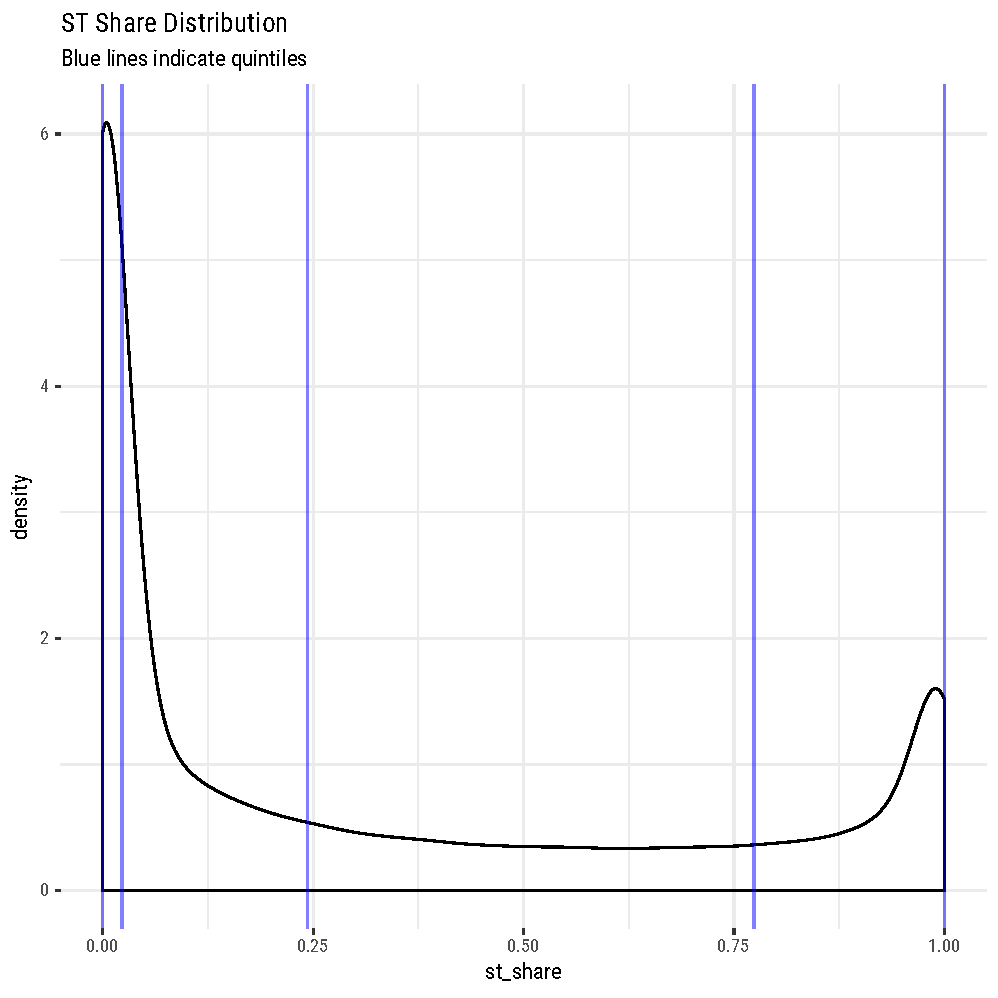
\includegraphics[width=4 in,angle=0]{Output/st_share_density.pdf}}
\smallskip
\scriptsize
\emph{Notes}: 
\end{minipage}
\end{center}
\end{figure}



\pagebreak
\subsection{Mining analysis}
\begin{figure}[htbp!]
\begin{center}
\begin{minipage}{1 \linewidth}
  \caption{\textbf{Balance in pre-treatment deforestation}}
  \label{fig:panelmatchbal}	
\centerline{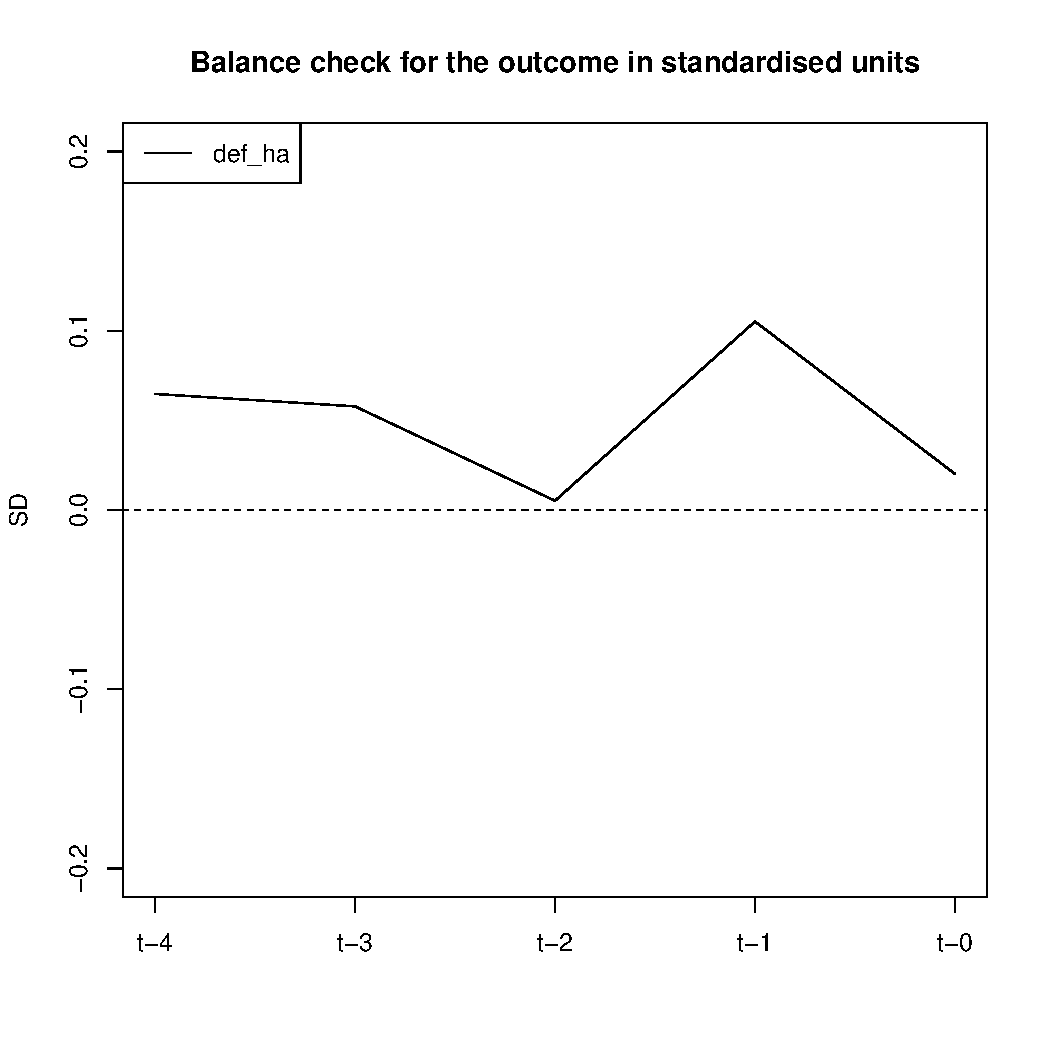
\includegraphics[width=4 in,angle=0]{Output/PanelMatch_bal.pdf}}
\smallskip
\scriptsize
\emph{Notes}: 
\end{minipage}
\end{center}
\end{figure}



\begin{figure}
  \centering
  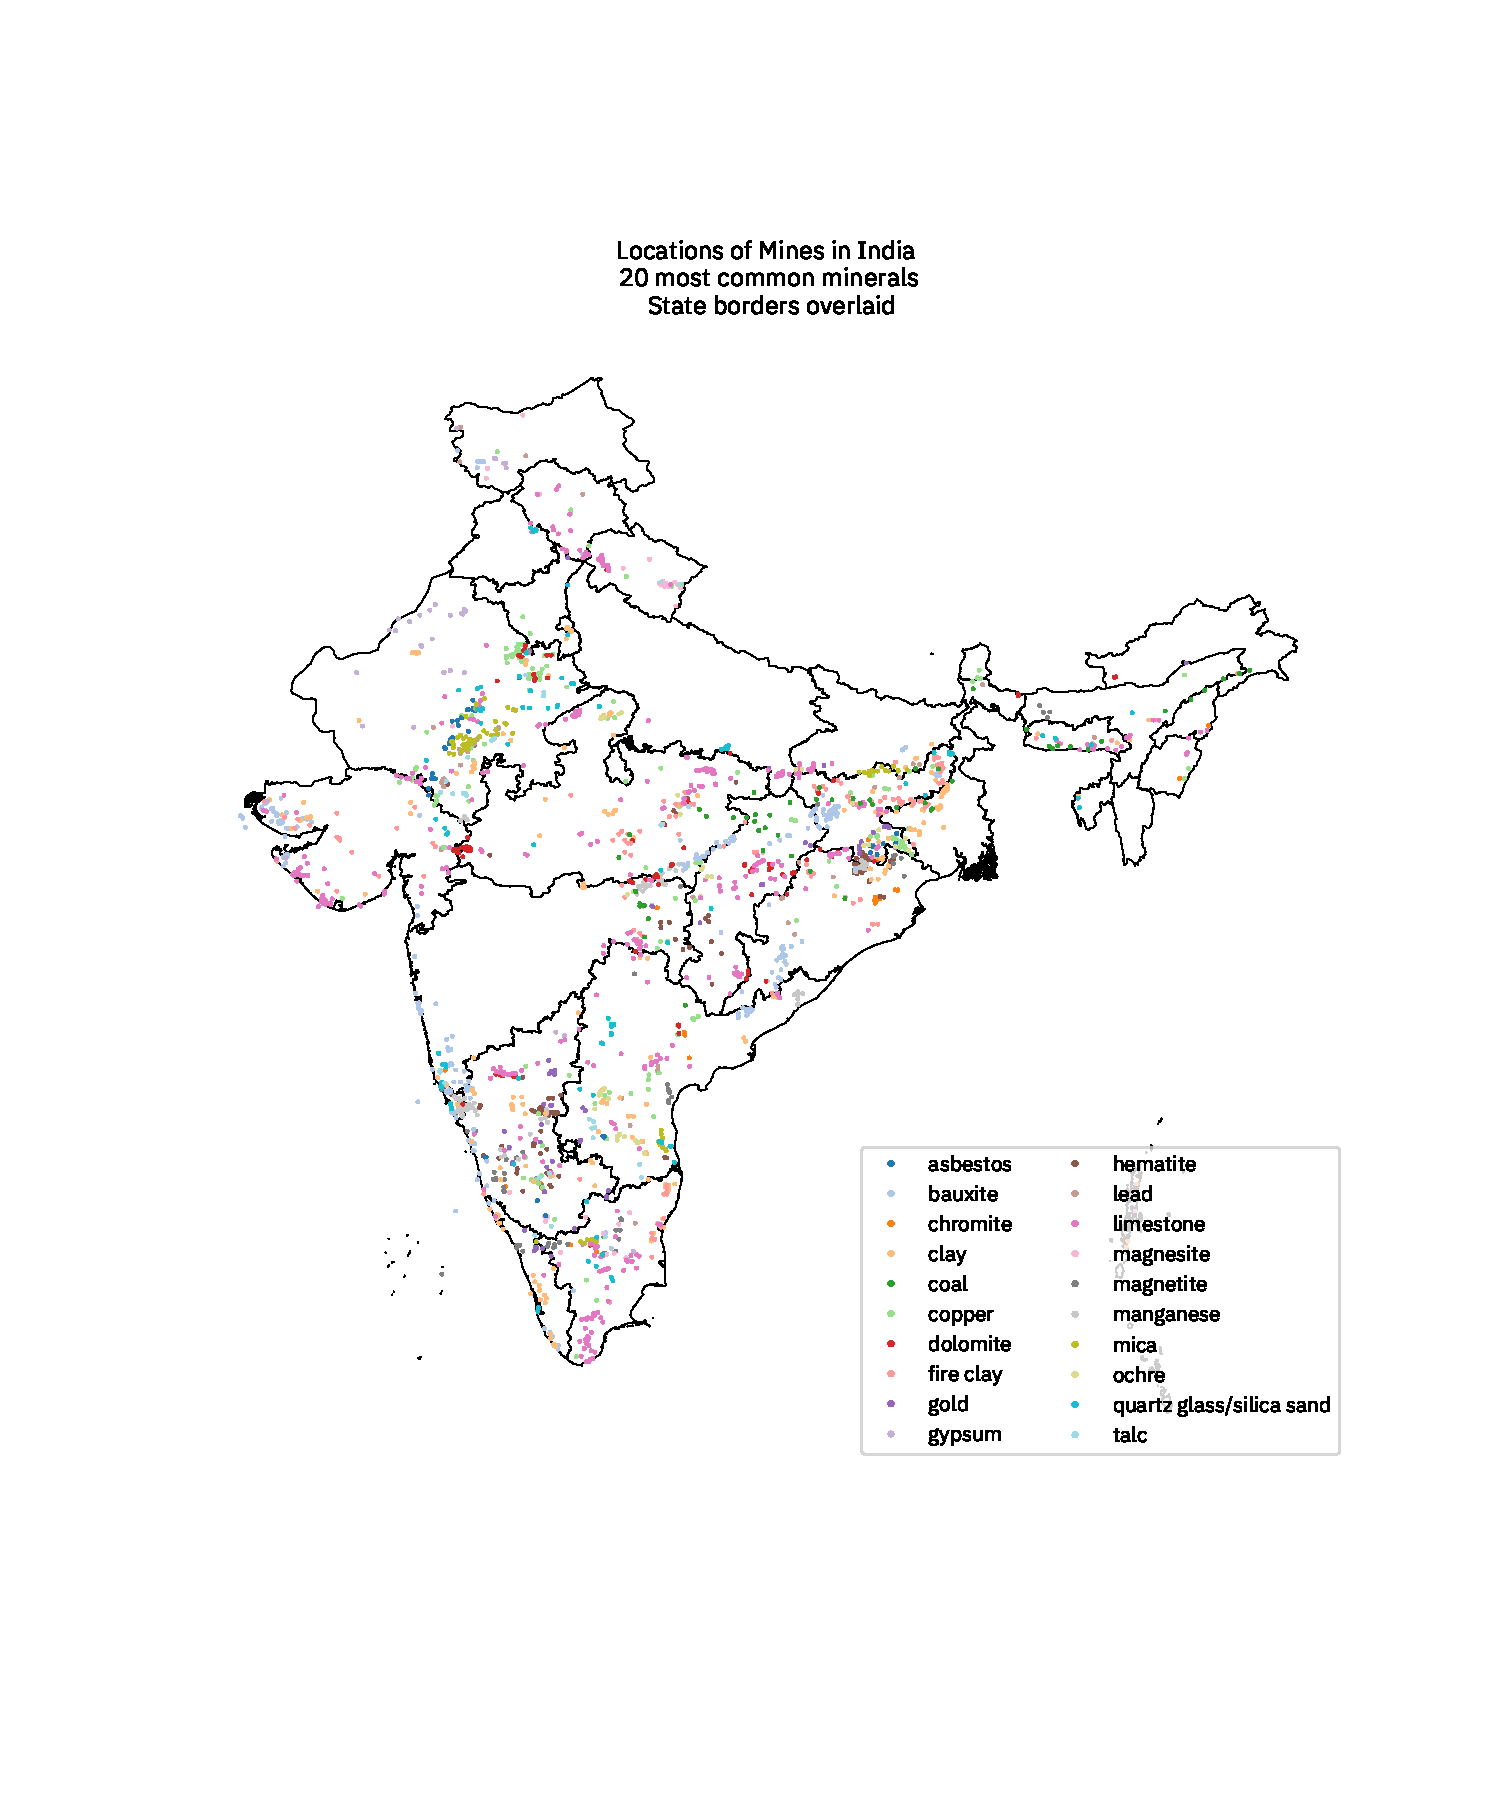
\includegraphics[]{Output/mine_map.pdf}
  \caption{Location of 20 most common minerals}
  \label{fig:mine_map}
\end{figure}

\begin{figure}
  \centering
  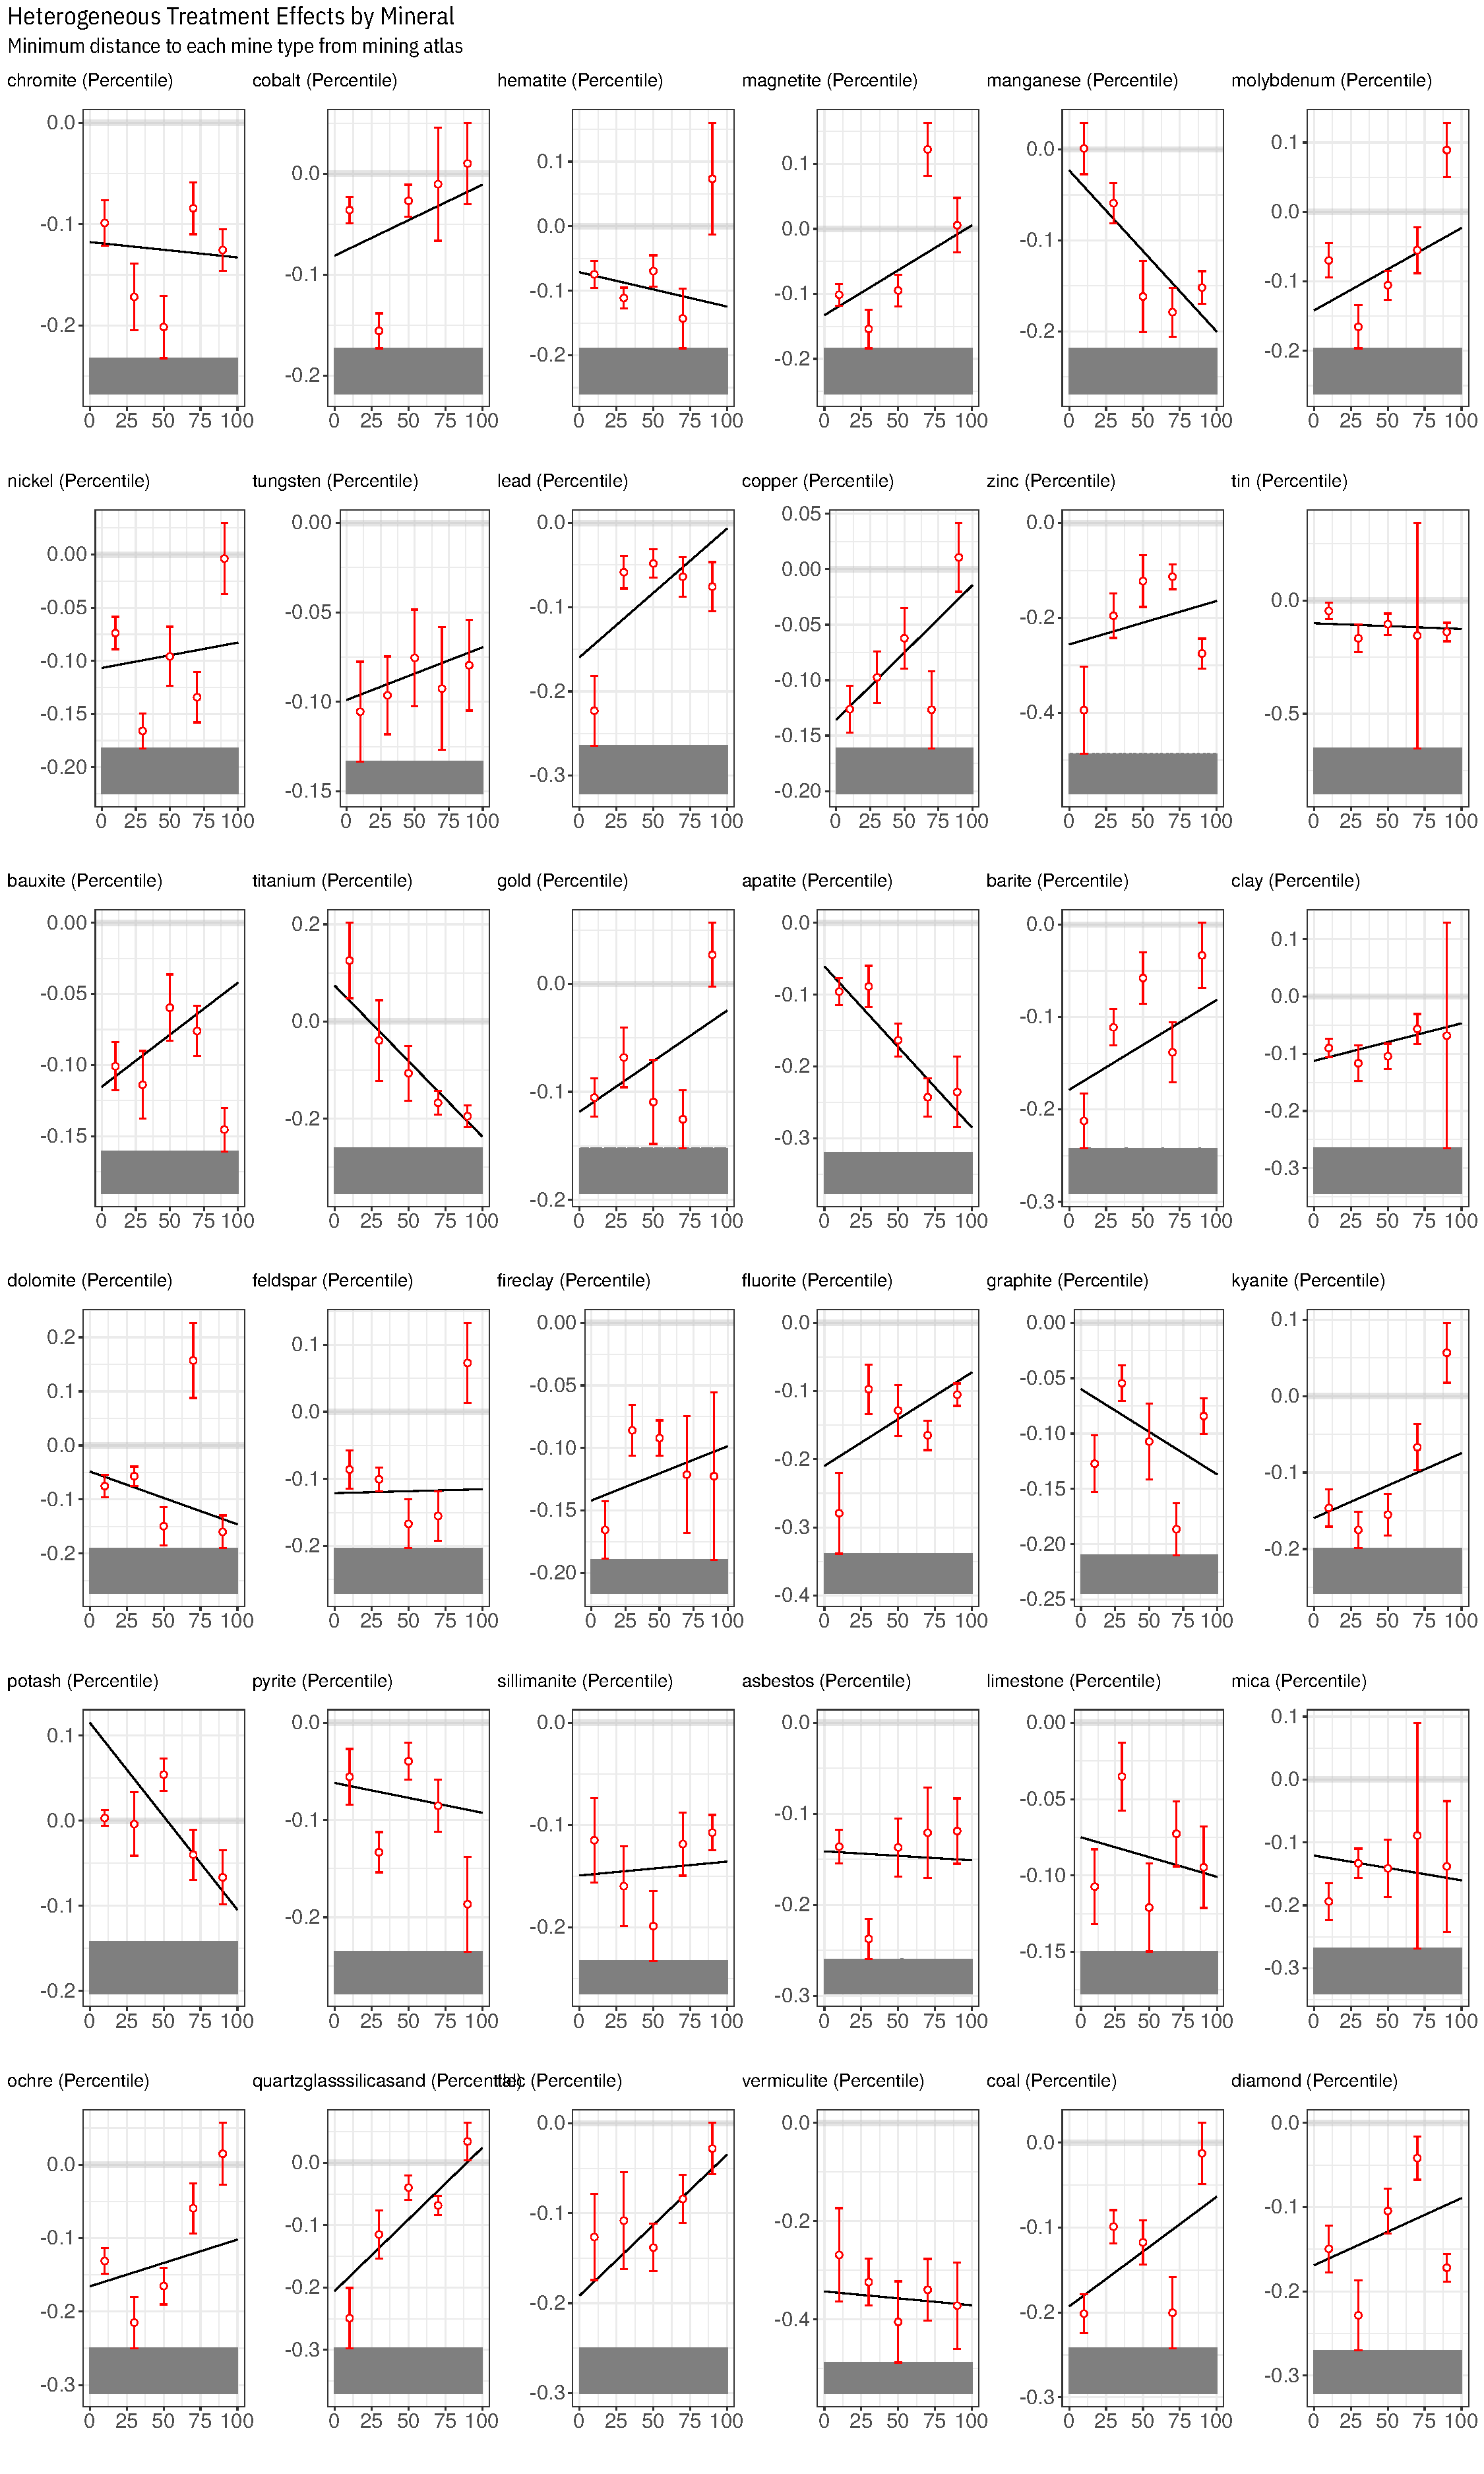
\includegraphics[]{Output/mining_het_te.pdf}
  \caption{Interaction effects by mine type}
  \label{fig:mine_het_te}
\end{figure}





%%%%%%%%%%%%%%%%%%%%%%%%%%%%%%%%%%%%%%%%%%%%%%%%%%%%%%%%%%%%%%%
\end{document}
